\documentclass[11pt,compress,t,notes=noshow, xcolor=table, aspectratio=169]{beamer}
\usepackage[]{graphicx}

\usepackage[]{color}
% maxwidth is the original width if it is less than linewidth
% otherwise use linewidth (to make sure the graphics do not exceed the margin)
\makeatletter
\def\maxwidth{ %
  \ifdim\Gin@nat@width>\linewidth
    \linewidth
  \else
    \Gin@nat@width
  \fi
}
\makeatother

\definecolor{fgcolor}{rgb}{0.345, 0.345, 0.345}
\newcommand{\hlnum}[1]{\textcolor[rgb]{0.686,0.059,0.569}{#1}}%
\newcommand{\hlstr}[1]{\textcolor[rgb]{0.192,0.494,0.8}{#1}}%
\newcommand{\hlcom}[1]{\textcolor[rgb]{0.678,0.584,0.686}{\textit{#1}}}%
\newcommand{\hlopt}[1]{\textcolor[rgb]{0,0,0}{#1}}%
\newcommand{\hlstd}[1]{\textcolor[rgb]{0.345,0.345,0.345}{#1}}%
\newcommand{\hlkwa}[1]{\textcolor[rgb]{0.161,0.373,0.58}{\textbf{#1}}}%
\newcommand{\hlkwb}[1]{\textcolor[rgb]{0.69,0.353,0.396}{#1}}%
\newcommand{\hlkwc}[1]{\textcolor[rgb]{0.333,0.667,0.333}{#1}}%
\newcommand{\hlkwd}[1]{\textcolor[rgb]{0.737,0.353,0.396}{\textbf{#1}}}%
\let\hlipl\hlkwb

\usepackage{framed}
\makeatletter
\newenvironment{kframe}{%
 \def\at@end@of@kframe{}%
 \ifinner\ifhmode%
  \def\at@end@of@kframe{\end{minipage}}%
  \begin{minipage}{\columnwidth}%
 \fi\fi%
 \def\FrameCommand##1{\hskip\@totalleftmargin \hskip-\fboxsep
 \colorbox{shadecolor}{##1}\hskip-\fboxsep
     % There is no \\@totalrightmargin, so:
     \hskip-\linewidth \hskip-\@totalleftmargin \hskip\columnwidth}%
 \MakeFramed {\advance\hsize-\width
   \@totalleftmargin\z@ \linewidth\hsize
   \@setminipage}}%
 {\par\unskip\endMakeFramed%
 \at@end@of@kframe}
\makeatother

\definecolor{shadecolor}{rgb}{.97, .97, .97}
\definecolor{messagecolor}{rgb}{0, 0, 0}
\definecolor{warningcolor}{rgb}{1, 0, 1}
\definecolor{errorcolor}{rgb}{1, 0, 0}
\newenvironment{knitrout}{}{} % an empty environment to be redefined in TeX

\newcommand{\SweaveOpts}[1]{}  % do not interfere with LaTeX
\newcommand{\SweaveInput}[1]{} % because they are not real TeX commands
\newcommand{\Sexpr}[1]{}       % will only be parsed by R
\newcommand{\xmark}{\ding{55}}%

\usepackage{alltt}
\usepackage[utf8]{inputenc}

\usepackage[english]{babel}
\usepackage{dsfont}
\usepackage{verbatim}
\usepackage{amsmath}
\usepackage{amsfonts}
\usepackage{amssymb}
\usepackage{bm}
\usepackage{csquotes}
\usepackage{multirow}
\usepackage{longtable}
\usepackage{booktabs}
\usepackage{enumerate}
\usepackage[absolute,overlay]{textpos}
\usepackage{psfrag}
\usepackage{algorithm}
\usepackage{algpseudocode}
\usepackage{eqnarray}
\usepackage{arydshln}
\usepackage{tabularx}
\usepackage{placeins}
\usepackage{tikz}
\usepackage{setspace}
\usepackage{colortbl}
\usepackage{mathtools}
\usepackage{wrapfig}
\usepackage{bm}
\usepackage{amsmath}
\usepackage{pifont}
\usepackage{xcolor} %colored math symbols
\usepackage{adjustbox}
\usepackage{verbatimbox}
\usepackage{tcolorbox}
\usepackage{siunitx}
\def\signed #1{{\leavevmode\unskip\nobreak\hfil\penalty50\hskip1em
  \hbox{}\nobreak\hfill #1%
  \parfillskip=0pt \finalhyphendemerits=0 \endgraf}}

% basic latex stuff
\newcommand{\col}{\par\colorbox{code}{\parbox{\textwidth}{\theverbbox}}\par}


\usetikzlibrary{shapes,arrows,automata,positioning,calc,chains,trees, shadows}
\tikzset{
  %Define standard arrow tip
  >=stealth',
  %Define style for boxes
  punkt/.style={
    rectangle,
    rounded corners,
    draw=black, very thick,
    text width=6.5em,
    minimum height=2em,
    text centered},
  % Define arrow style
  pil/.style={
    ->,
    thick,
    shorten <=2pt,
    shorten >=2pt,}
}

\newsavebox\mybox
\newenvironment{aquote}[1]
  {\savebox\mybox{#1}\begin{quote}\openautoquote\hspace*{-.7ex}}
  {\unskip\closeautoquote\vspace*{1mm}\signed{\usebox\mybox}\end{quote}}

\usepackage{subfig}

% Defines macros and environments
\usepackage{../style/dhbw-lecture}


\let\code=\texttt
\let\proglang=\textsf

\setkeys{Gin}{width=0.9\textwidth}

% The accent rule sits on its own vbox line with \nointerlineskip so it costs
% only its own 1.2pt height + the explicit 2pt gap, instead of pulling in a
% full \baselineskip (~0.6-0.7cm) the way a plain "\\" line break would --
% that overhead on every single frame is what was pushing picture-heavy
% frames over the shorter 16:9 frame height.
\setbeamertemplate{frametitle}{\expandafter\uppercase\expandafter\insertframetitle\par\vskip2pt\nointerlineskip\hbox{\color{dhbwaccent}\rule{1.6cm}{1.2pt}}}
\addtobeamertemplate{frametitle}{}{\vspace{0.08cm}}

\usepackage{bbm}
% basic latex stuff
\newcommand{\pkg}[1]{{\fontseries{b}\selectfont #1}} %fontstyle for R packages
\newcommand{\lz}{\vspace{0.5cm}} %vertical space
\newcommand{\dlz}{\vspace{1cm}} %double vertical space
\newcommand{\oneliner}[1] % Oneliner for important statements
{\begin{block}{}\begin{center}\begin{Large}#1\end{Large}\end{center}\end{block}}


%new environments
\newenvironment{vbframe}  %frame with breaks and verbatim
{
 \begin{frame}[containsverbatim,allowframebreaks]
}
{
\end{frame}
}

\newenvironment{vframe}  %frame with verbatim without breaks (to avoid numbering one slided frames)
{
 \begin{frame}[containsverbatim]
}
{
\end{frame}
}

\newenvironment{blocki}[1]   % itemize block
{
 \begin{block}{#1}\begin{itemize}
}
{
\end{itemize}\end{block}
}

\newenvironment{fragileframe}[2]{  %fragile frame with framebreaks
\begin{frame}[allowframebreaks, fragile, environment = fragileframe]
\frametitle{#1}
#2}
{\end{frame}}


\newcommand{\myframe}[2]{  %short for frame with framebreaks
\begin{frame}[allowframebreaks]
\frametitle{#1}
#2
\end{frame}}

\newcommand{\remark}[1]{
  \textbf{Remark:} #1
}


\newenvironment{deleteframe}
{
\begingroup
\usebackgroundtemplate{
\includegraphics[width=\paperwidth,height=\paperheight]{../style/color/red.png}}
 \begin{frame}
}
{
\end{frame}
\endgroup
}
\newenvironment{simplifyframe}
{
\begingroup
\usebackgroundtemplate{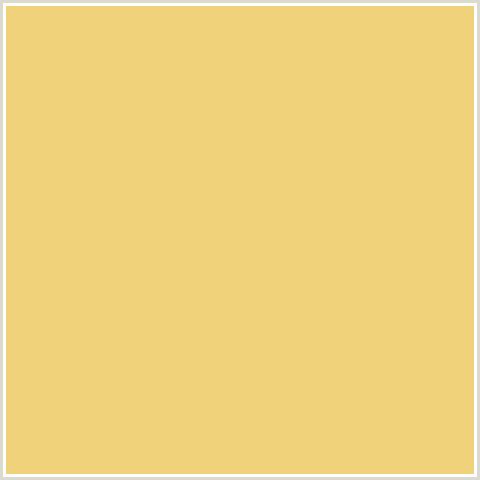
\includegraphics[width=\paperwidth,height=\paperheight]{../style/color/yellow.png}}
 \begin{frame}
}
{
\end{frame}
\endgroup
}\newenvironment{draftframe}
{
\begingroup
\usebackgroundtemplate{
\includegraphics[width=\paperwidth,height=\paperheight]{../style/color/green.jpg}}
 \begin{frame}
}
{
\end{frame}
\endgroup
}
% https://tex.stackexchange.com/a/261480: textcolor that works in mathmode
\makeatletter
\renewcommand*{\@textcolor}[3]{%
  \protect\leavevmode
  \begingroup
    \color#1{#2}#3%
  \endgroup
}
\makeatother


\input{../latex-math/basic-math}
\input{../latex-math/basic-ml}
\input{../latex-math/ml-nn}

\newcommand{\titlefigure}{figure/cortex.png}
\newcommand{\learninggoals}{
  \item CNNs as a locally-connected, weight-sharing alternative to fully-connected networks, suited to spatial and sequential data
  \item The convolution operation as a learned local feature detector, generalized to 1D, 2D, and 3D data (time series, images, video/volumetric data)
  \item Padding, stride, and input channels, and how they determine output feature map size
  \item Sparse connectivity, parameter sharing, and translation equivariance as the properties that make convolutions efficient
  \item Dilated and transposed convolutions, pooling, and how these ideas culminate in modern architectures (residual/skip connections)
}

\title{Advanced Artificial Intelligence and Machine Learning}
\date{}

\begin{document}

\lecturechapter{CNN}
\lecture{Advanced AI \& ML}
%%%%%%%%%%%%%%%%%%%%%%%%%%%%%%%%%%%%%%%%%%%%%%%%%%%%%%%%%%%%%%%%%%

\section{Basic Concepts}
%%%%%%%%%%%%%%%%%%%%%%%%%%%%%%%%%%%%%%%%%%%%%%%%%%%%%%%%%%%%%%%%%%

\begin{frame}{Convolutional Neural Networks}
\begin{itemize}
    \item CNNs are inspired by the biological visual cortex, where connectivity resembles the mammalian visual system.
    \item Since their breakthrough win of the 2012 ILSVRC competition, CNNs have become the dominant model class in computer vision.
    \item Common applications: image classification, object detection/localization, semantic segmentation --- plus, outside vision, NLP, audio, and time-series data.
    \item Basic idea: a CNN automatically extracts spatial (or, more generally, structured) features so a downstream layer can predict optimally.
    \item Like MLPs, CNNs are built from composable building blocks --- but with a different connectivity pattern, covered in this session.
\end{itemize}
\end{frame}
%%%%%%%%%%%%%%%%%%%%%%%%%%%%%%%%%%%%%%%%%%%%%%%%%%%%%%%%%%%%%%%%%%

\begin{frame}{Biological Inspiration}
\begin{figure}
\centering
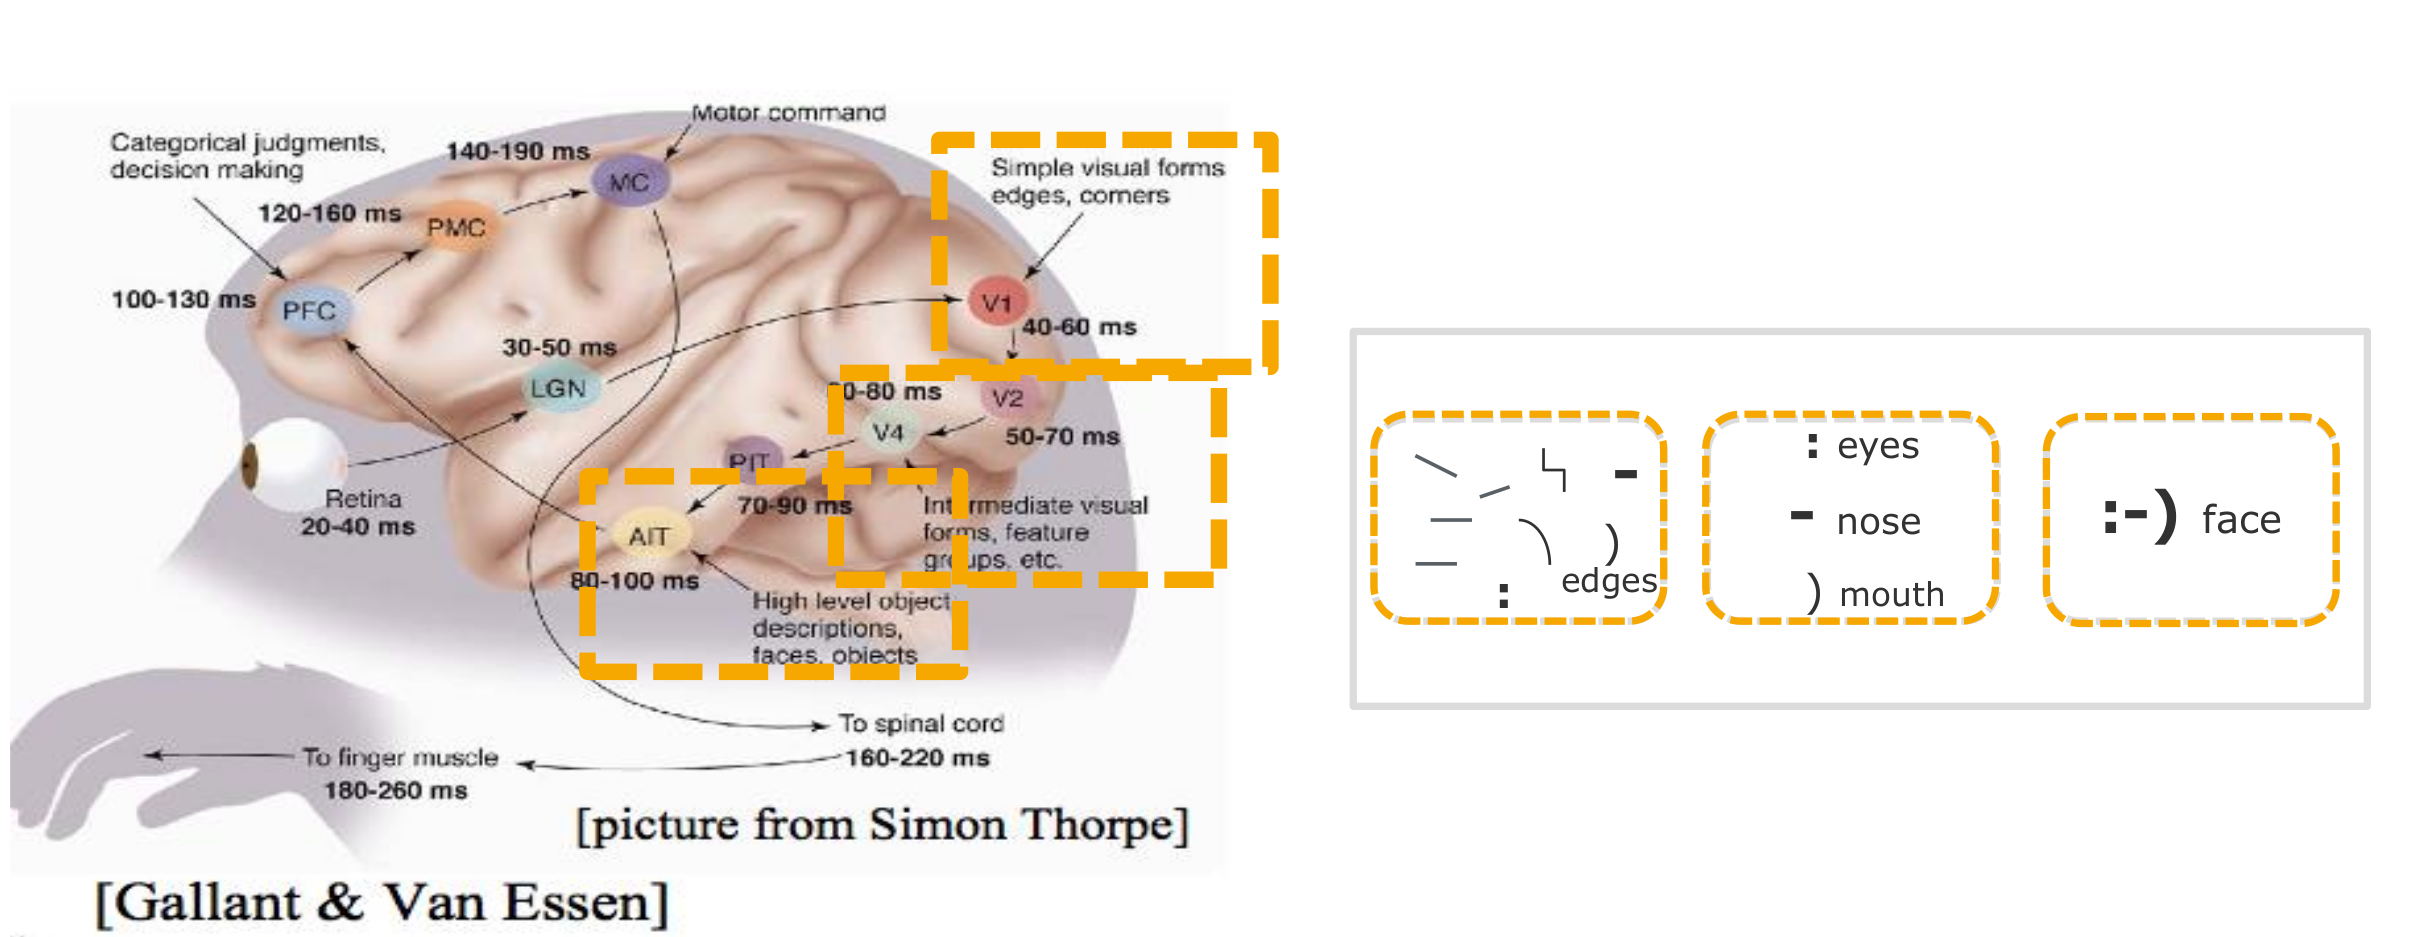
\includegraphics[width=8cm]{figure/cortex.png}
\caption{The ventral (recognition) pathway in the visual cortex has multiple stages --- Retina, LGN, V1, V2, V4, PIT, AIT, etc.\ --- consisting of many intermediate representations.}
\end{figure}
\end{frame}

%%%%%%%%%%%%%%%%%%%%%%%%%%%%%%%%%%%%%%%%%%%%%%%%%%%%%%%%%%%%%%%%%%

\begin{vbframe}{CNNs in the Real World}
  \begin{figure}
    \centering
    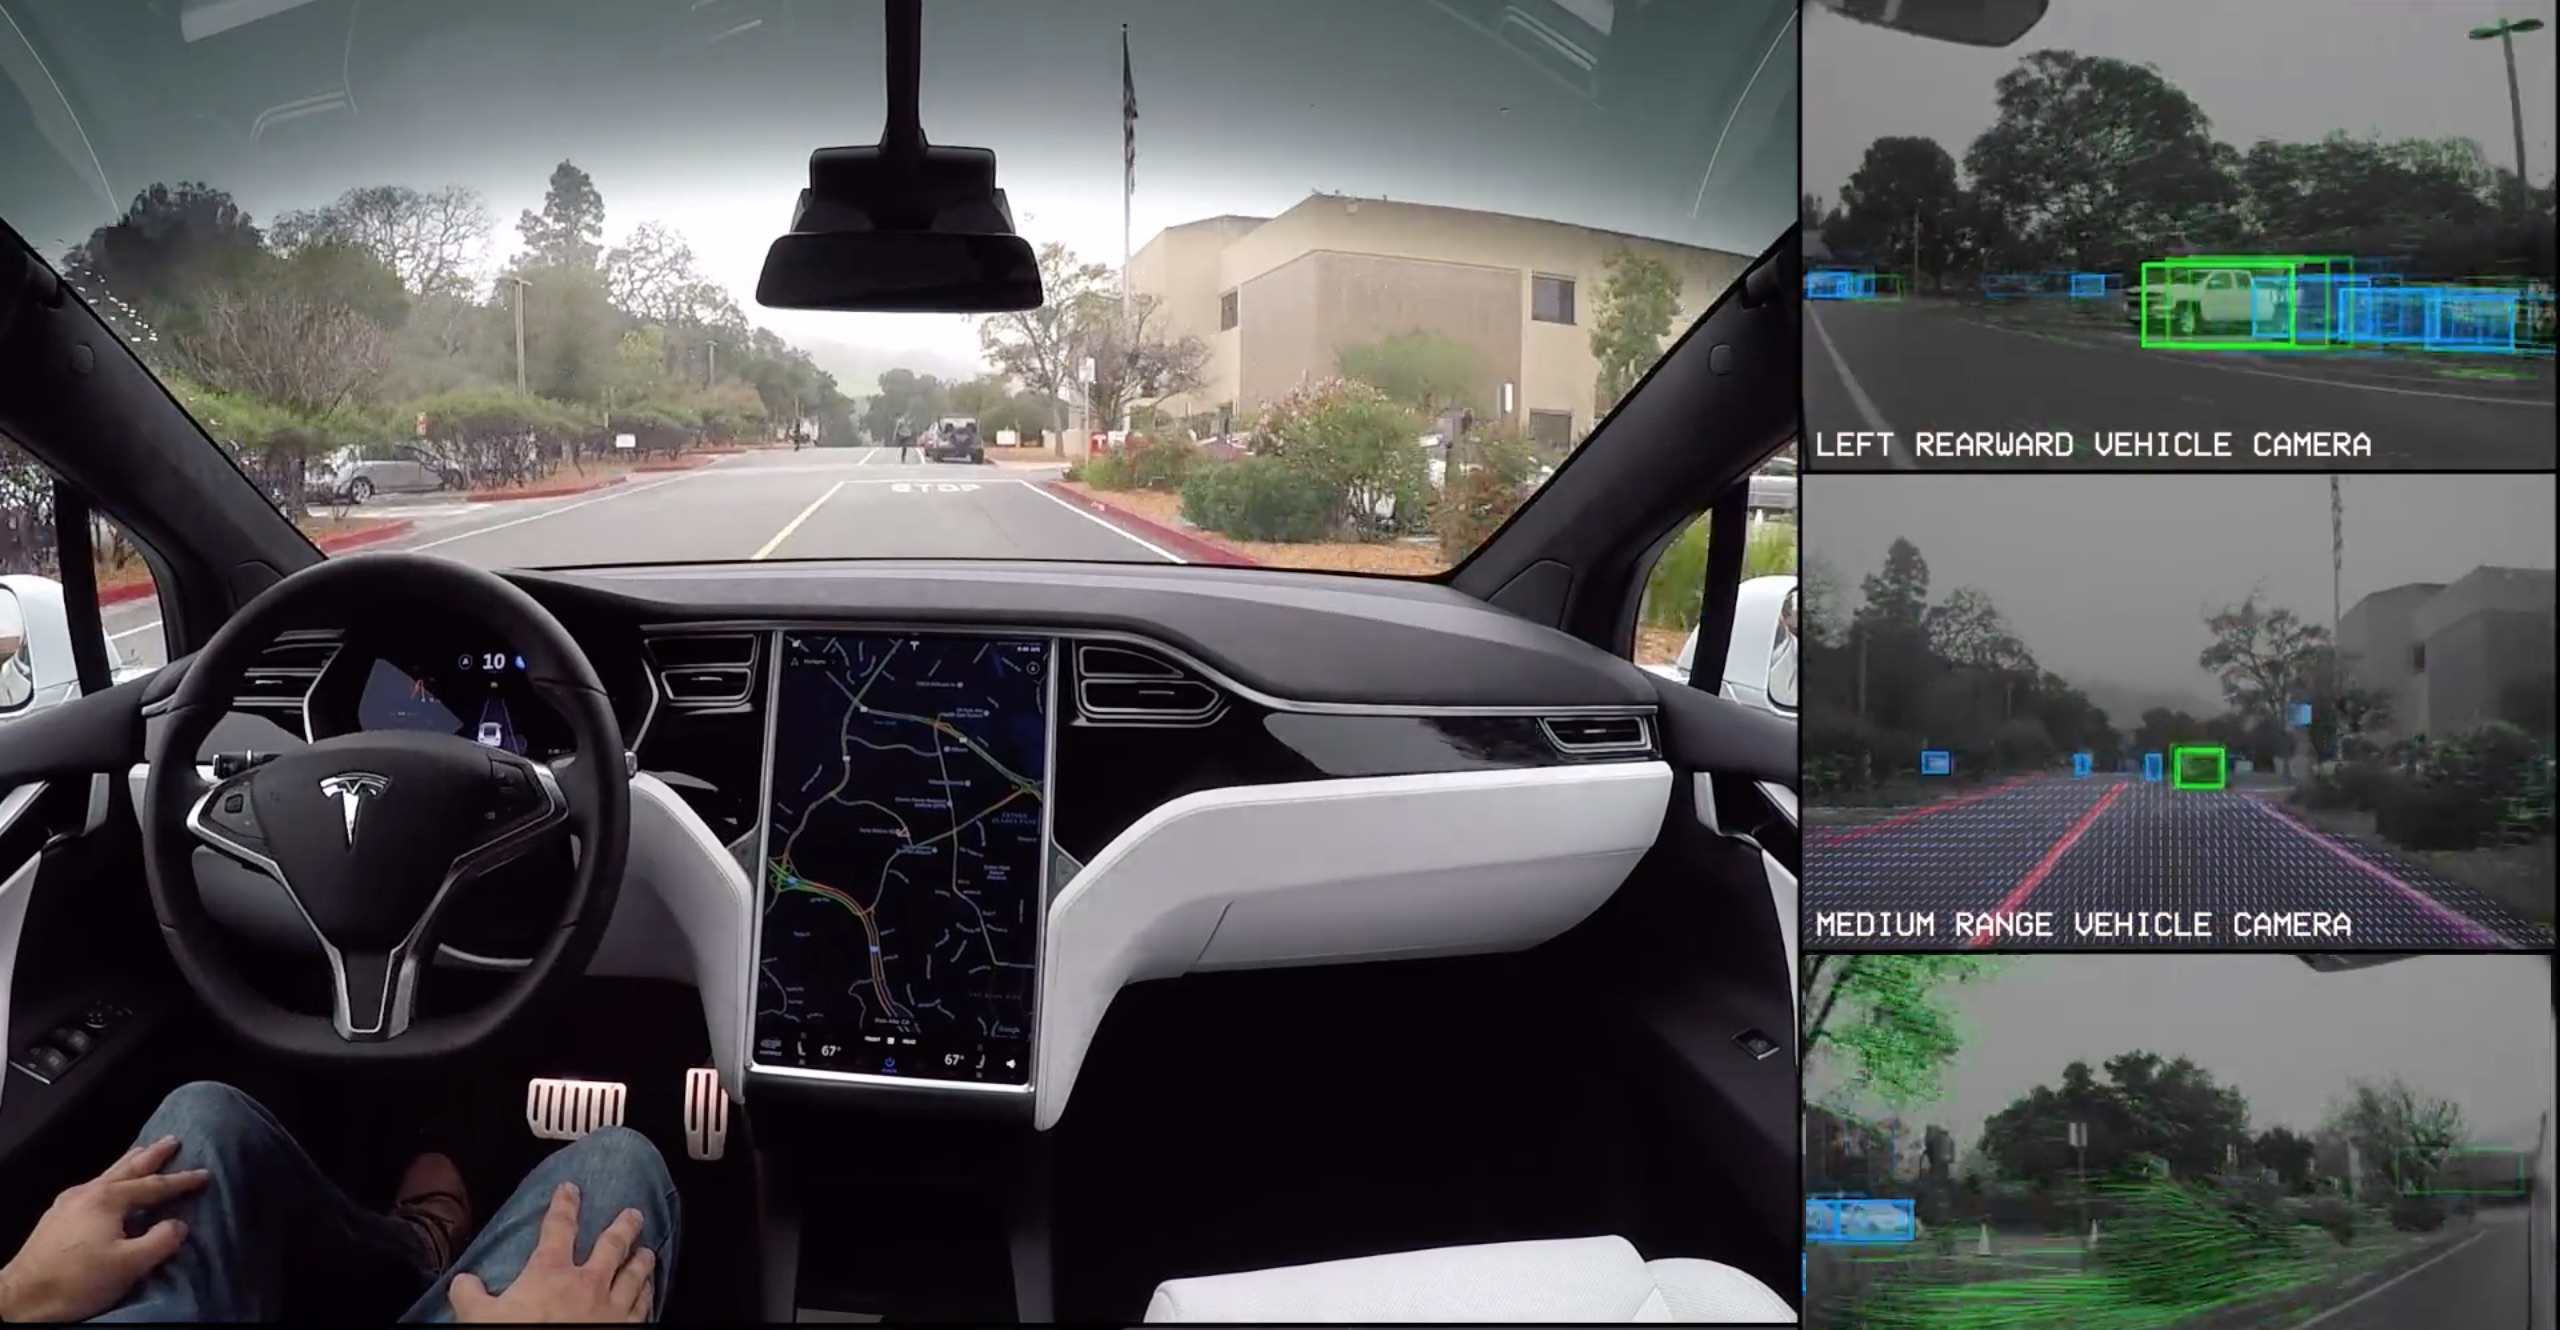
\includegraphics[width=7cm]{figure/tesla_autopilot.jpg}
    \caption{Self-driving: a CNN maps raw pixels from a single front-facing camera directly into steering commands, learning to drive in traffic, on marked and unmarked roads, and on highways (The Tesla Team, 2016).}
  \end{figure}
\framebreak
%%%%%%%%%%%%%%%%%%%%%%%%%%%%%%%%%%%%%%%%%%%%%%%%%%%%%%%%%%%%%%%%%%

\begin{figure}
    \centering
    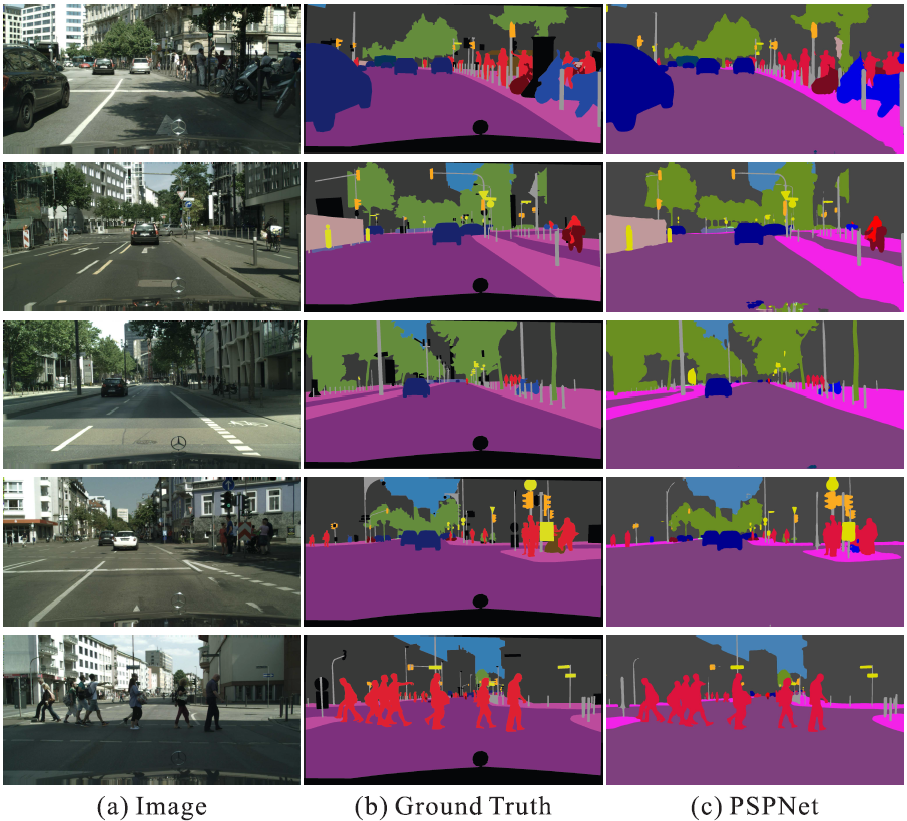
\includegraphics[width=6cm]{figure/cityscapes_visual.png}
    \caption{Semantic segmentation: a CNN extracts a feature map, a pyramid-parsing module harvests sub-region representations at multiple scales, and a final convolution produces a per-pixel class prediction (Zhao et al., 2017).}
  \end{figure}
\end{vbframe}
%%%%%%%%%%%%%%%%%%%%%%%%%%%%%%%%%%%%%%%%%%%%%%%%%%%%%%%%%%%%%%%%%%

\begin{frame}{CNNs --- A First Glimpse}
\center
\only<1>{\begin{figure} 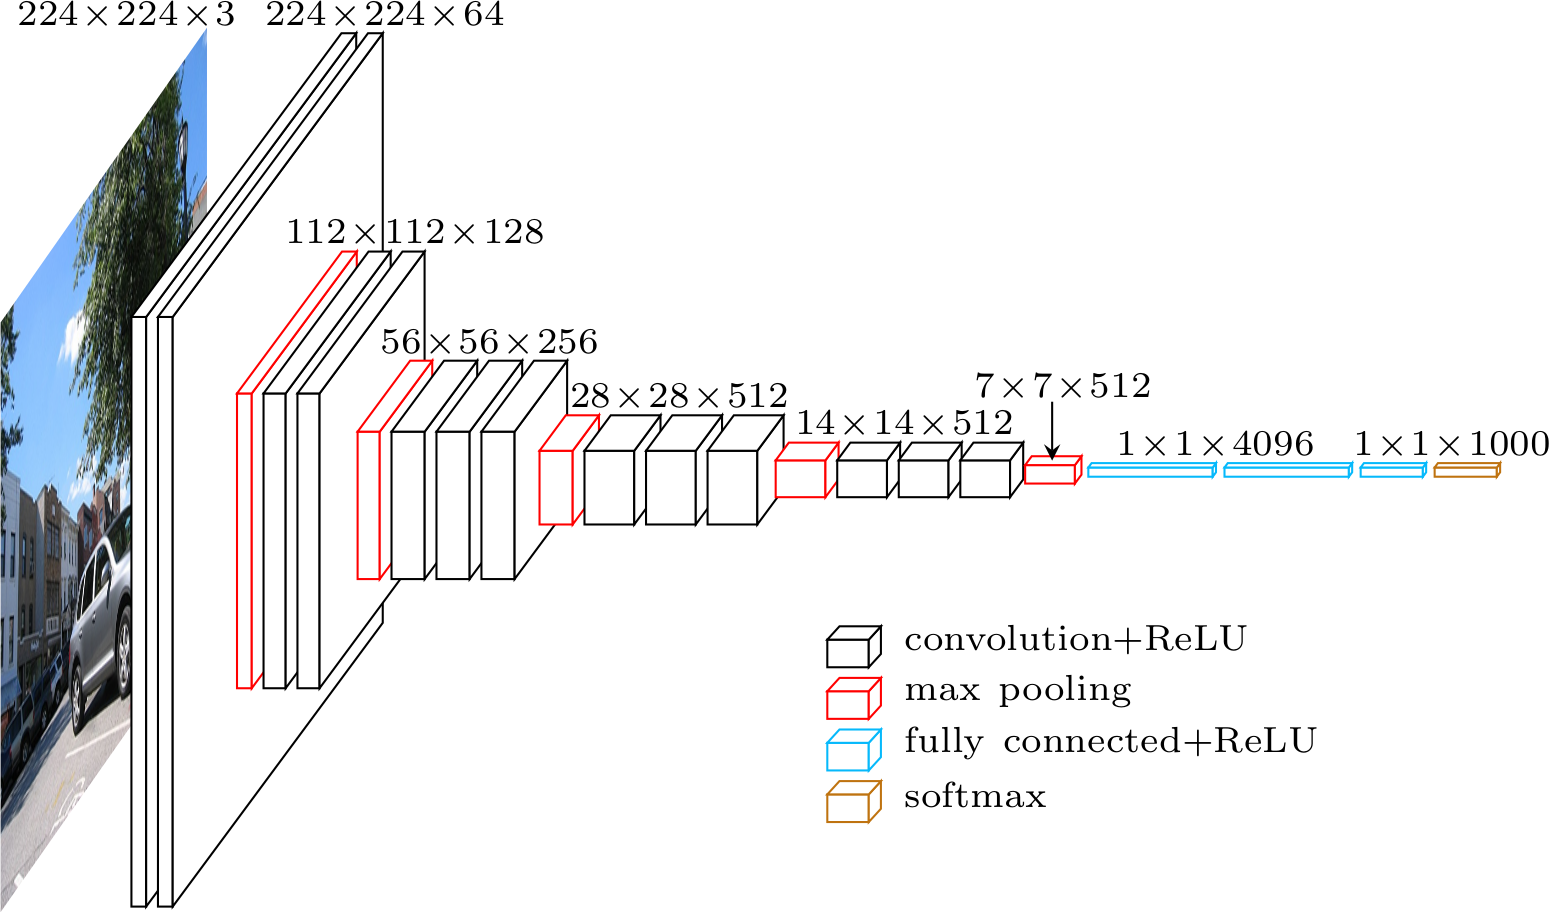
\includegraphics[width=8cm]{figure/alexnet.png}
\caption{Example CNN architecture, with typical layer types labeled.} \end{figure}}%
\only<2>{\begin{figure} 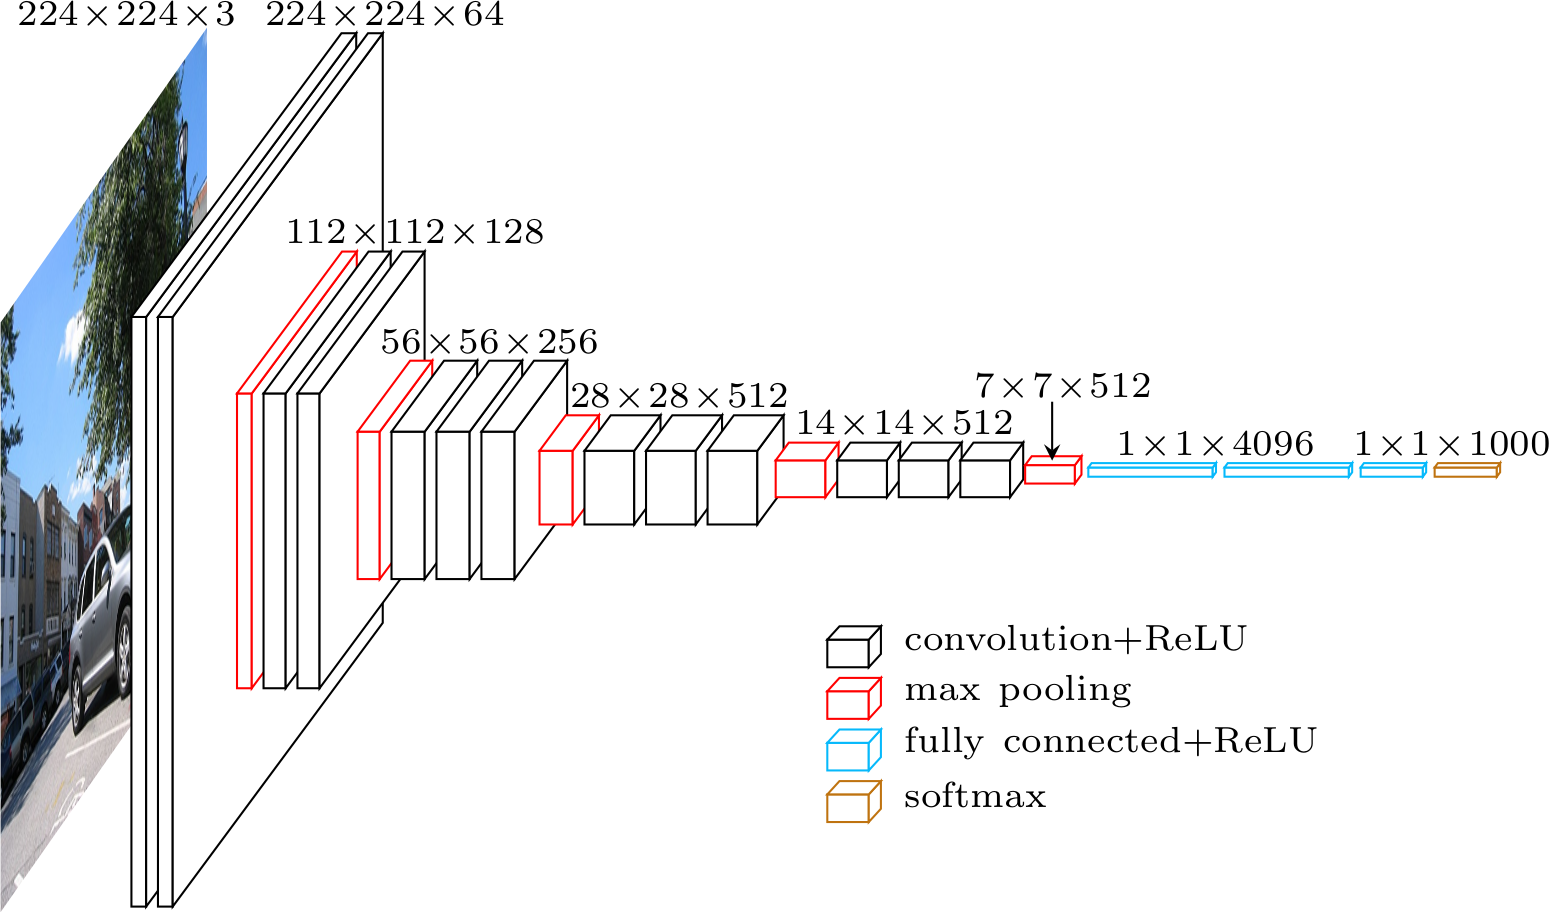
\includegraphics[width=8cm]{figure/alexnet.png}
\caption{Example CNN architecture, with typical layer types labeled.}\end{figure}}%
\begin{itemize}
\only<1>{\item \textbf{Input layer} takes the input data (e.g.\ image, audio).}
\only<1>{\item \textbf{Convolution layers} extract feature maps from the previous layer.}
\only<1>{\item \textbf{Pooling layers} reduce the dimensionality of feature maps and retain the most salient features.}
\only<2>{\item \textbf{Fully connected layers} connect feature-map elements to the output neurons.}
\only<2>{\item \textbf{Softmax} converts output values to class probabilities.}
\end{itemize}
\end{frame}
%%%%%%%%%%%%%%%%%%%%%%%%%%%%%%%%%%%%%%%%%%%%%%%%%%%%%%%%%%%%%%%%%%
%%%%%%%%%%%%%%%%%%          REFERENCES          %%%%%%%%%%%%%%%%%%
%%%%%%%%%%%%%%%%%%%%%%%%%%%%%%%%%%%%%%%%%%%%%%%%%%%%%%%%%%%%%%%%%%
\begin{vbframe}
\frametitle{References}
\footnotesize{
\begin{thebibliography}{99}
\bibitem[(The Tesla Team, 2016)]{1} The Tesla Team. (2016, October 19). \textit{All Tesla cars being produced now have full self-driving hardware: Tesla Switzerland}. Tesla. \url{https://www.tesla.com/de_ch/blog/all-tesla-cars-being-produced-now-have-full-self-driving-hardware}
\bibitem[(Zhao et al., 2017)]{2} Zhao, H., Shi, J., Qi, X., Wang, X., \& Jia, J. (2017, July). \textit{Pyramid Scene Parsing Network}. Proceedings of the IEEE Conference on Computer Vision and Pattern Recognition (CVPR).
\end{thebibliography}
}
\end{vbframe}

%%%%%%%%%%%%%%%%%%%%%%%%%%%%%%%%%%%%%%%%%%%%%%%%%%%%%%%%%%%%%%%%%%
\section{The Convolution Operation}
%%%%%%%%%%%%%%%%%%%%%%%%%%%%%%%%%%%%%%%%%%%%%%%%%%%%%%%%%%%%%%%%%%

\begin{vbframe}{Filters to Extract Features}
    \begin{itemize}
        \item Filters have been used in computer vision since the 1970s.
        \item One prominent example: the \textbf{Sobel filter}, which detects edges in images.
    \end{itemize}
    \begin{figure}
        \centering
        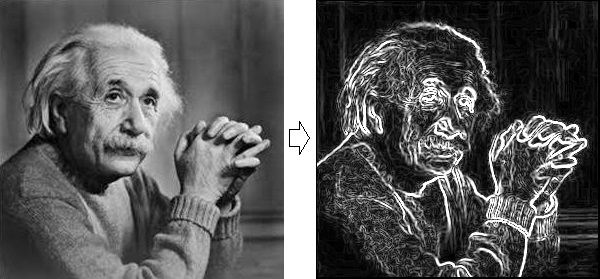
\includegraphics[width=10cm]{figure/sobel_einstein.png}
        \caption{Sobel-filtered image (Qmegas, 2016).}
    \end{figure}
\framebreak
%%%%%%%%%%%%%%%%%%%%%%%%%%%%%%%%%%%%%%%%%%%%%%%%%%%%%%%%%%%%%%%%%%

\begin{itemize}
\item Edges occur where pixel intensity changes rapidly over neighboring pixels, so we approximate the intensity gradient at each pixel.
\item Sobel showed that the gradient image $\textbf{G}_x$ of an original image $\textbf{A}$ in the $x$-dimension can be approximated by:
$$ \textbf{G}_x =
\begin{bmatrix}
-1 & 0 & +1 \\
-2 & 0 & +2 \\
-1 & 0 & +1
\end{bmatrix} * \textbf{A} = \textbf{S}_x * \textbf{A}
$$
where $*$ denotes a \textbf{convolution}, not ordinary matrix multiplication.
\item The filter matrix $\textbf{S}_x$ is the product of an \textbf{averaging} and a \textbf{differentiation} kernel:
$$
\underbrace{\begin{bmatrix}
1 & 2 & 1
\end{bmatrix}^{T}}_{averaging}
\underbrace{\begin{bmatrix}
-1 & 0 & +1
\end{bmatrix}}_{differentiation}
$$
\end{itemize}
\framebreak
%%%%%%%%%%%%%%%%%%%%%%%%%%%%%%%%%%%%%%%%%%%%%%%%%%%%%%%%%%%%%%%%%%
    \begin{itemize}
        \item Similarly, the gradient image $\textbf{G}_y$ in the $y$-dimension is approximated by:
        $$
            \textbf{G}_y =
            \begin{bmatrix}
                -1 & -2 & -1  \\
                0 & 0 & 0 \\
                +1 & +2 & +1
            \end{bmatrix} * \textbf{A} = \textbf{S}_y * \textbf{A}
        $$
        \item Combining both gradient images yields a direction-independent gradient magnitude $\textbf{G}$:
        $$
            \textbf{G} = \sqrt{\textbf{G}_x^2 + \textbf{G}_y^2}
        $$
    \end{itemize}
\end{vbframe}
%%%%%%%%%%%%%%%%%%%%%%%%%%%%%%%%%%%%%%%%%%%%%%%%%%%%%%%%%%%%%%%%%%

\begin{frame}{Horizontal vs.\ Vertical Edges}
    \begin{figure}
        \centering
          \scalebox{0.8}{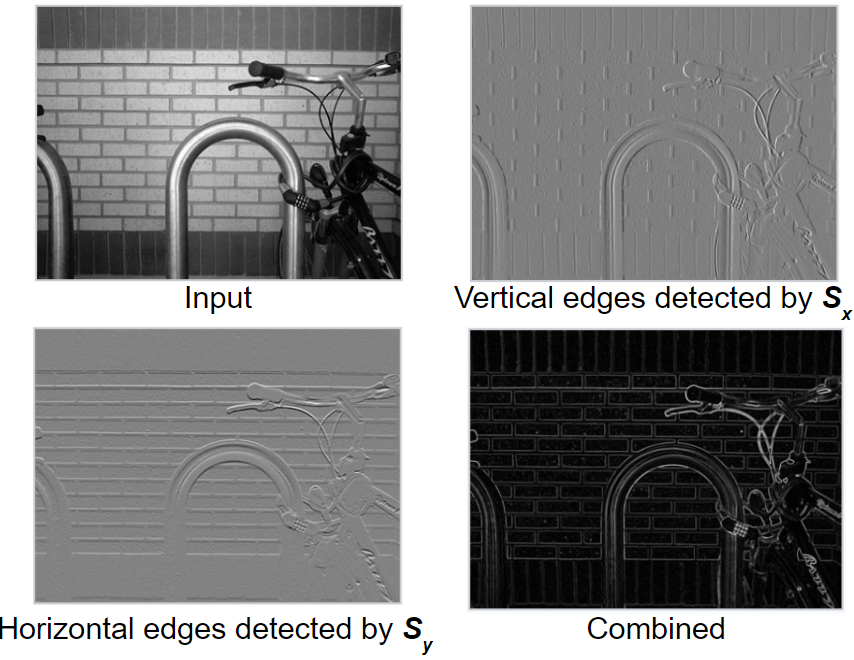
\includegraphics{figure/sobel_bike.png}}
         \caption{Sobel-filtered images, normalized per direction (Wikipedia, 2022).}
    \end{figure}
\end{frame}
%%%%%%%%%%%%%%%%%%%%%%%%%%%%%%%%%%%%%%%%%%%%%%%%%%%%%%%%%%%%%%%%%%

\begin{frame}{Filters to Extract Features}
    \center
    \only<1>{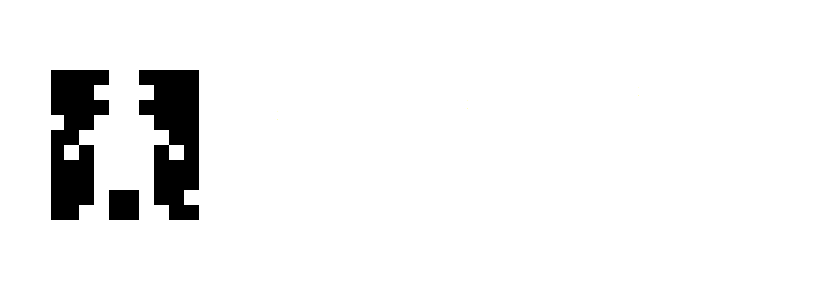
\includegraphics[width=11cm]{figure/sobel1.png}}%
    \only<2>{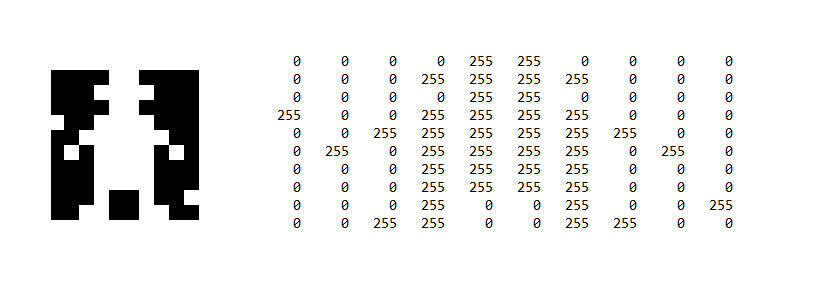
\includegraphics[width=11cm]{figure/sobel2.png}}%
    \only<3>{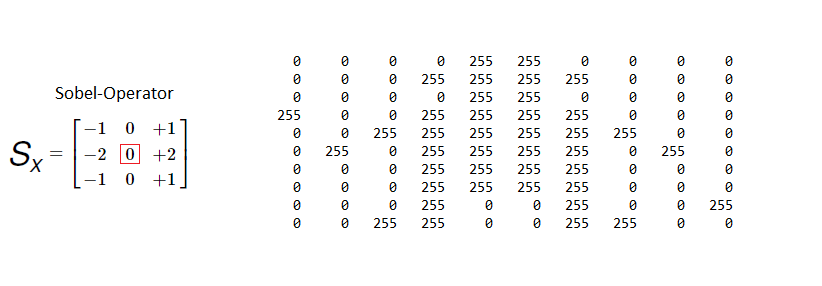
\includegraphics[width=11cm]{figure/sobel3.png}}%
    \only<4>{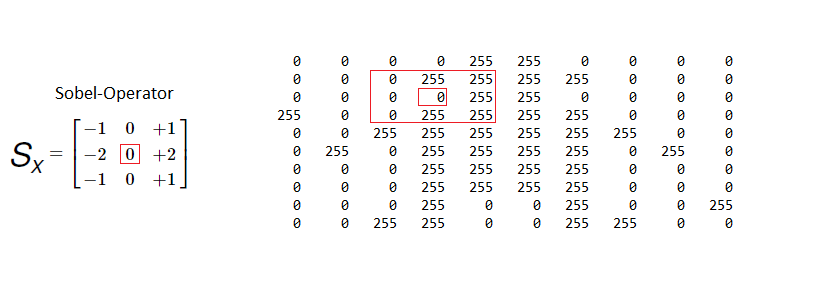
\includegraphics[width=11cm]{figure/sobel4.png}}%
    \only<5>{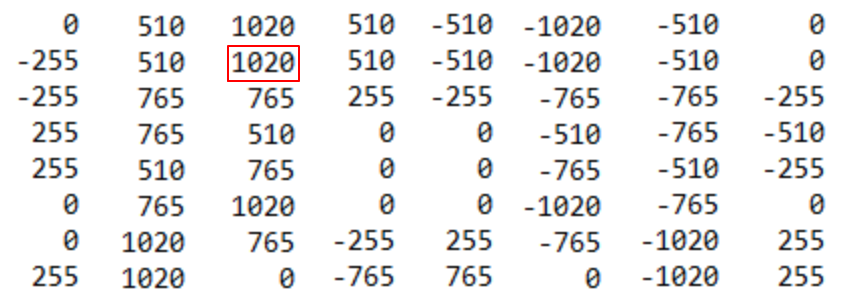
\includegraphics[width=6cm]{figure/sobel6.png}}%
    \only<6>{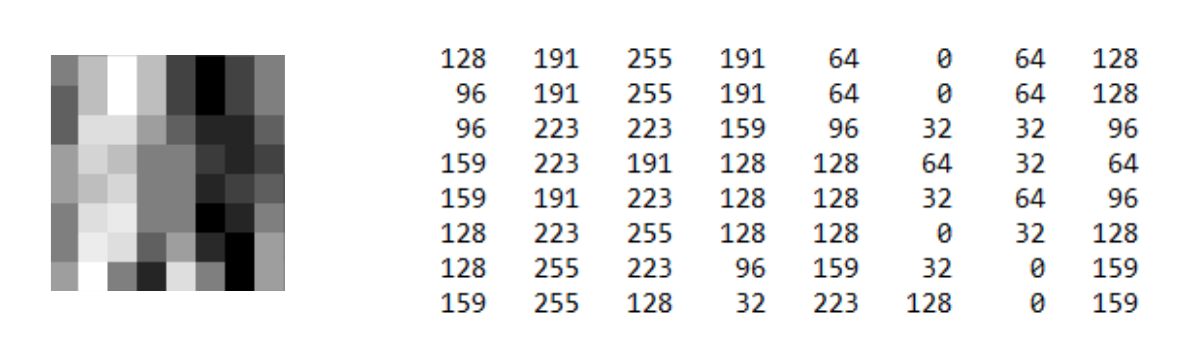
\includegraphics[width=11cm]{figure/sobel8.png}}%

    \begin{itemize}
        \only<1>{\item Let's apply this to a small dummy image --- how do we represent a digital image?}
        \only<2>{\item Basically as an array of integers.}
        \only<3>{\item $\textbf{S}_x$ lets us detect vertical edges.}
        \only<4>{\item[]
        \vspace{-0.8cm}
        \begin{alignat*}{3}
            (\textbf{G}_x)_{(i,j)} = (\textbf{I} \star \textbf{S}_x)_{(i, j)}
                 & = -1 \cdot 0 \ \ &&+ \ \ 0 \cdot 255 \ \ &&+ \ \ \textbf{1} \cdot \textbf{255} \\
                 &\quad - 2 \cdot 0 &&+ \ \ 0 \cdot 0 &&+ \ \ \textbf{2} \cdot \textbf{255} \\
                 &\quad - 1 \cdot 0 &&+ \ \ 0 \cdot 255 &&+ \ \ \textbf{1} \cdot \textbf{255}
                 \notag
        \end{alignat*}
        }
        \only<5>{\item Applying the Sobel operator at every location in the input yields the \textbf{feature map}.}
        \only<6>{\item Normalized, the feature map reveals vertical edges. Note the dimensional reduction compared to the input.}
    \end{itemize}
\end{frame}

%%%%%%%%%%%%%%%%%%%%%%%%%%%%%%%%%%%%%%%%%%%%%%%%%%%%%%%%%%%%%%%%%%
\begin{vbframe}{Why Does This Matter for CNNs?}
  \begin{itemize}
    \item What we just did was extract a \textbf{pre-defined} feature from the input (edges).
    \item A CNN does almost exactly the same thing: it extracts features from the input --- the key difference is that we do not tell it what to look for; \textbf{the network learns the filters itself}.
    \item In a nutshell:
    \begin{itemize}
      \item Initialize many random filters (like the Sobel filter, but with random entries) and apply them to the input.
      \item Feed the resulting feature maps into a classifier (e.g.\ a feedforward net).
      \item Update the filter entries via gradient descent, exactly like any other weight.
    \end{itemize}
  \end{itemize}
\end{vbframe}
%%%%%%%%%%%%%%%%%%%%%%%%%%%%%%%%%%%%%%%%%%%%%%%%%%%%%%%%%%%%%%%%%%

\begin{frame}{The 2D Convolution}
\begin{itemize}
\only<1-8>{\item Suppose we have an input with entries $a, b, \dots, i$ (think: pixel values).}
\only<1-8>{\item The filter we apply has weights $w_{11}, w_{12}, w_{21}$, and $w_{22}$.}
\end{itemize}
\center
\only<1>{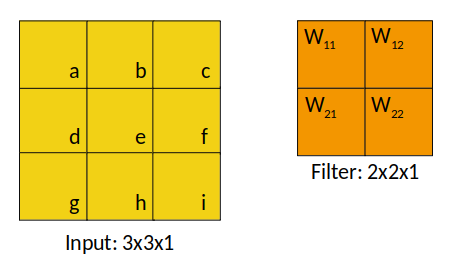
\includegraphics[width=7cm]{figure/conv2d_1.png}}%
\only<2>{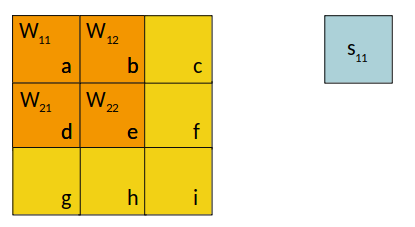
\includegraphics[width=6cm]{figure/conv2d_2.png}}%
\only<3>{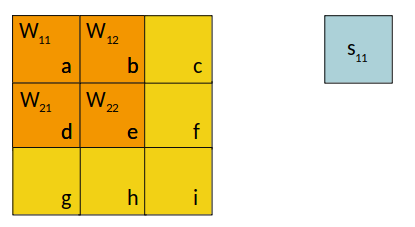
\includegraphics[width=6cm]{figure/conv2d_2.png}}%
\only<4>{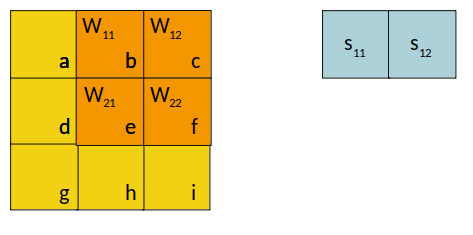
\includegraphics[width=7cm]{figure/conv2d_3.png}}%
\only<5>{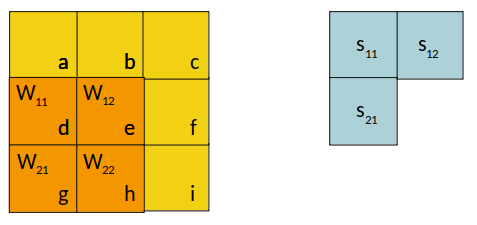
\includegraphics[width=7cm]{figure/conv2d_4.png}}%
\only<6>{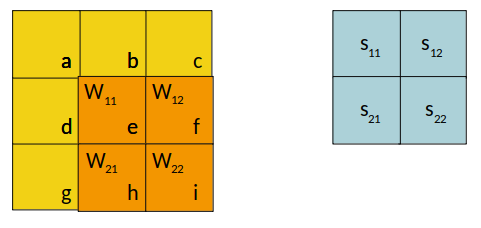
\includegraphics[width=7cm]{figure/conv2d_5.png}}%
\only<7>{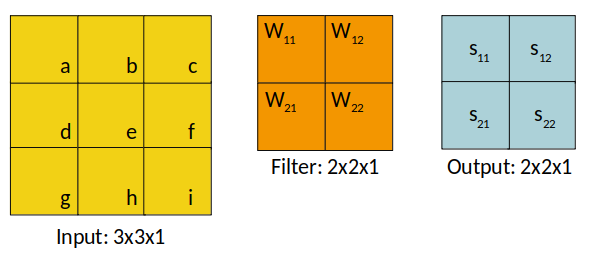
\includegraphics[width=8cm]{figure/conv2d_6.png}}%
\only<8>{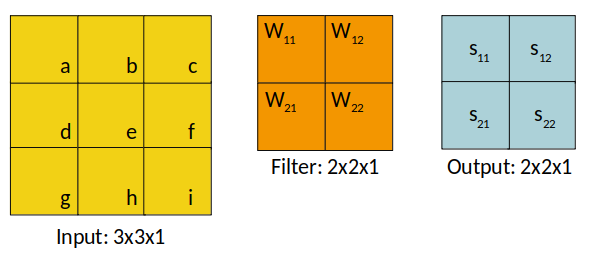
\includegraphics[width=8cm]{figure/conv2d_6.png}}%

\begin{itemize}
\only<1>{\item[] }
\only<2>{\item[] }
\only<3>{\item[] To obtain $s_{11}$ we compute the dot product: $s_{11} = a \cdot w_{11} + b \cdot w_{12} + d \cdot w_{21} + e \cdot w_{22}$}
\only<4>{\item[] Same for $s_{12}$: $s_{12} = b \cdot w_{11} + c \cdot w_{12} + e \cdot w_{21} + f \cdot w_{22}$}
\only<5>{\item[] As well as for $s_{21}$: $s_{21} = d \cdot w_{11} + e \cdot w_{12} + g \cdot w_{21} + h \cdot w_{22}$}
\only<6>{\item[] And finally for $s_{22}$: $s_{22} = e \cdot w_{11} + f \cdot w_{12} + h \cdot w_{21} + i \cdot w_{22}$}
\only<7>{\item[] All four entries together give the full $2\times 2$ output feature map.}
\only<8>{\item[] More generally, let $I$ be the input matrix and $W$ the filter/kernel. Then the output entries are $s_{ij} = \sum_{m,n} I_{i+m-1, j+n-1} \, w_{mn}$, with $m,n$ ranging over the filter size.}
\end{itemize}
\end{frame}
%%%%%%%%%%%%%%%%%%%%%%%%%%%%%%%%%%%%%%%%%%%%%%%%%%%%%%%%%%%%%%%%%%

\begin{frame}{Working with Images}
  \begin{itemize}
  \item Grey-scale images: a matrix of dimension $\text{height} \times \text{width} \times 1$, with pixel values from $0$ (black) to $255$ (white).
  \item Color images: a tensor of dimension $\text{height} \times \text{width} \times 3$, where the depth $3$ denotes the RGB channels.
  \item A filter's depth is \textbf{always} equal to the input's depth. In practice, filters are usually square, so a single integer defines their spatial size --- e.g.\ a filter of size $2$ on a color image has dimensions $2\times 2\times 3$.
  \end{itemize}
\end{frame}
%%%%%%%%%%%%%%%%%%%%%%%%%%%%%%%%%%%%%%%%%%%%%%%%%%%%%%%%%%%%%%%%%%
%%%%%%%%%%%%%%%%%%          REFERENCES          %%%%%%%%%%%%%%%%%%
%%%%%%%%%%%%%%%%%%%%%%%%%%%%%%%%%%%%%%%%%%%%%%%%%%%%%%%%%%%%%%%%%%
\begin{vbframe}
\frametitle{References}
\footnotesize{
\begin{thebibliography}{99}
\bibitem[(Qmegas, 2016)]{1} Qmegas. (2016). \textit{QMEGAS/Sobel-Operator: PHP implementation of Sobel Operator (Sobel filter)}. GitHub. \url{https://github.com/qmegas/sobel-operator}
\bibitem[(Wikipedia, 2022)]{2} Wikimedia Foundation. (2022, September 1). \textit{Kantendetektion}. Wikipedia. \url{https://de.wikipedia.org/wiki/Kantendetektion}
\end{thebibliography}
}
\end{vbframe}

%%%%%%%%%%%%%%%%%%%%%%%%%%%%%%%%%%%%%%%%%%%%%%%%%%%%%%%%%%%%%%%%%%
\section{1D / 2D / 3D Convolutions}
%%%%%%%%%%%%%%%%%%%%%%%%%%%%%%%%%%%%%%%%%%%%%%%%%%%%%%%%%%%%%%%%%%

\begin{vbframe}{1D Convolutions}
\textbf{Data situation}: sequential, 1-dimensional tensor data.

\begin{itemize}
\item Data consists of tensors with shape [depth, xdim].
\item Depth $1$ (single-channel): univariate time series (e.g.\ a stock price over time), or functional/curve data.
\item Depth $> 1$ (multi-channel): multivariate time series (e.g.\ multi-sensor human activity recognition, temperature + humidity in weather forecasting), or text encoded as character-level one-hot vectors.
\end{itemize}

$\to$ Convolve the data with a 1D kernel.
\end{vbframe}
%%%%%%%%%%%%%%%%%%%%%%%%%%%%%%%%%%%%%%%%%%%%%%

\begin{vbframe}{1D Convolutions --- Operation}
    \begin{figure}
        \centering
        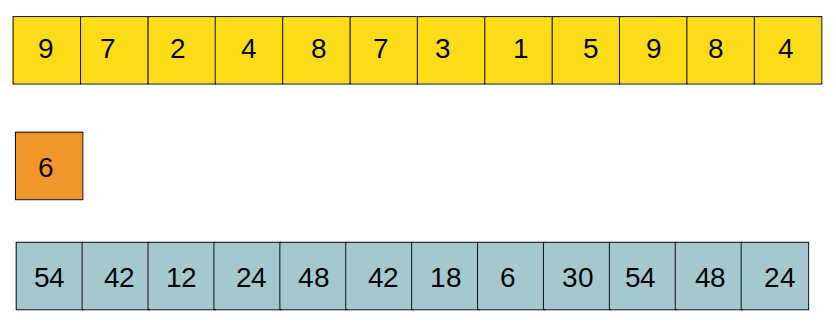
\includegraphics[width=10cm]{figure/conv1d-1.png}
        \caption{1D movement data with depth $1$ and filter size $1$.}
    \end{figure}
\framebreak
    \begin{figure}
        \centering
        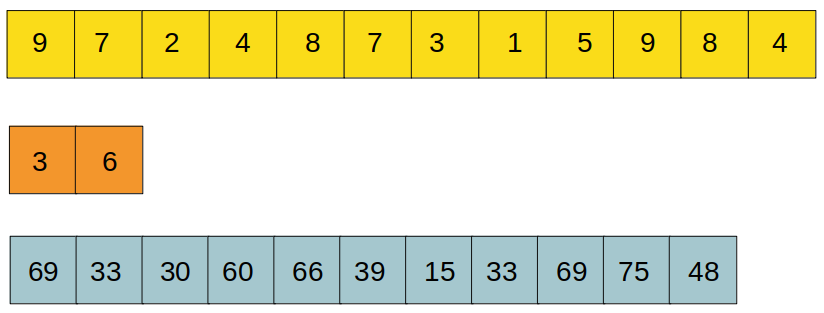
\includegraphics[width=10cm]{figure/conv1d-2.png}
        \caption{1D movement data with depth $1$ and filter size $2$.}
    \end{figure}
\end{vbframe}
%%%%%%%%%%%%%%%%%%%%%%%%%%%%%%%%%%%%%%%%%%%%%%%%%%

\begin{frame}{1D Convolutions --- Sensor and Time-Series Data}
    \begin{figure}
        \centering
        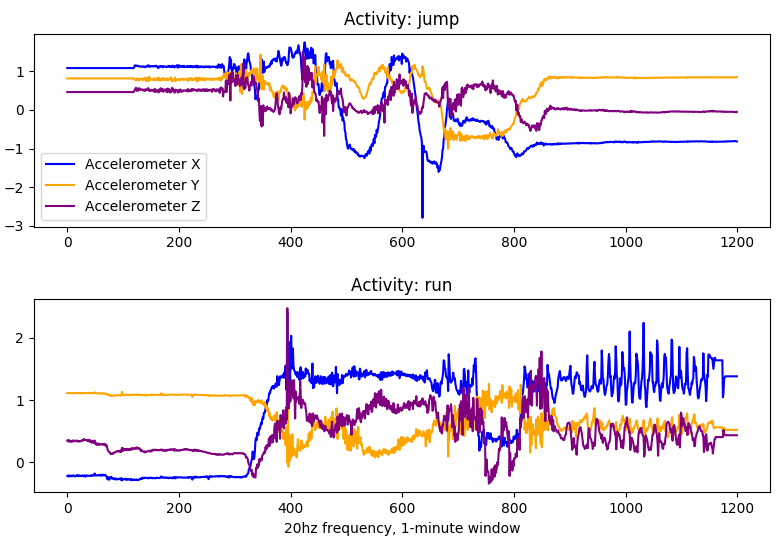
\includegraphics[width=9cm]{figure/HAR.png}
        \caption{1D movement data with depth $3$, measured by an accelerometer for human activity recognition.}
    \end{figure}
\end{frame}
%%%%%%%%%%%%%%%%%%%%%%%%%%%%%%%%%%%%%%%%%%%%%%%%%%%%%

\begin{frame}{1D Convolutions --- Sensor and Time-Series Data}
    \begin{figure}
        \centering
        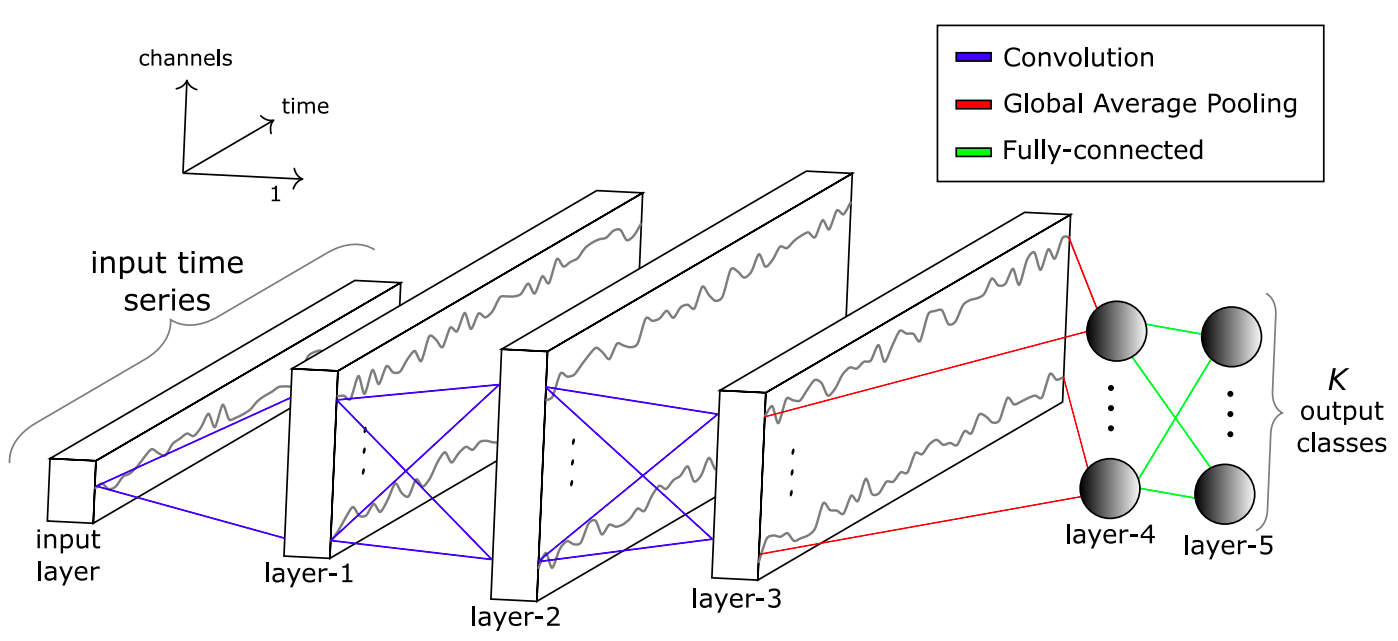
\includegraphics[width=10cm]{figure/deep_tsc.png}
        \caption{\footnotesize Time-series classification with a 1D CNN and global average pooling: an input series is convolved by 3 CNN layers, pooled, and fed into a dense layer before the softmax --- a classic time-series classification architecture (Ismail Fawaz et al., 2019).}
    \end{figure}
\end{frame}
%%%%%%%%%%%%%%%%%%%%%%%%%%%%%%%%%%%%%%%%%%%%%%%%%%%%%

\begin{vbframe}{1D Convolutions --- Text Mining}
    \begin{itemize}
        \item 1D convolutions also apply to text: e.g.\ classifying the sentiment of text snippets such as Yelp reviews.
    \end{itemize}
    \begin{figure}
        \centering
        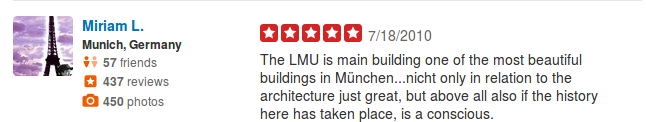
\includegraphics[width=12cm]{figure/yelp_lmu.png}
        \caption{Sentiment classification: is this a positive review?}
    \end{figure}
\end{vbframe}
%%%%%%%%%%%%%%%%%%%%%%%%%%%%%%%%%%%%%%%%%%%%%%%%

\frame{
\frametitle{1D Convolutions --- Text Mining}
    \center
    \only<1>{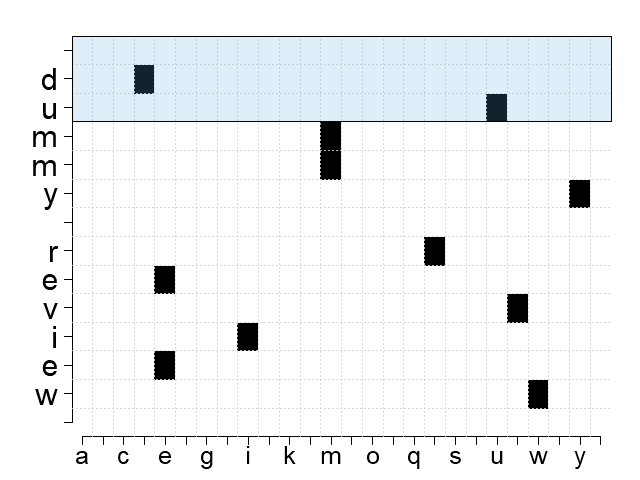
\includegraphics[width=5cm]{figure/1_encoded_text.png}}%
    \only<2>{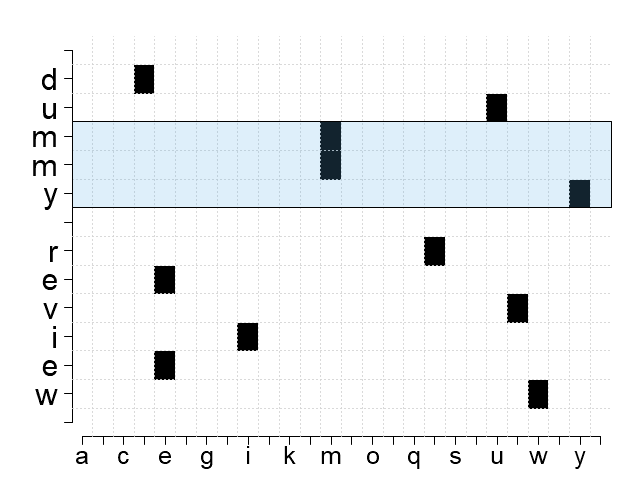
\includegraphics[width=9cm]{figure/4_encoded_text.png}}%
    \only<3>{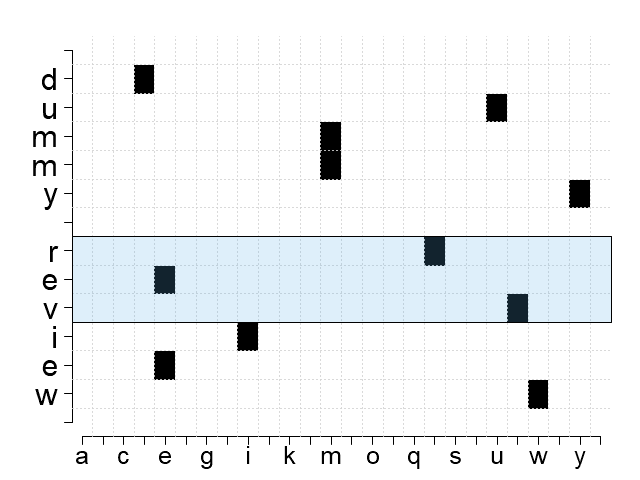
\includegraphics[width=9cm]{figure/8_encoded_text.png}}%
    \only<4>{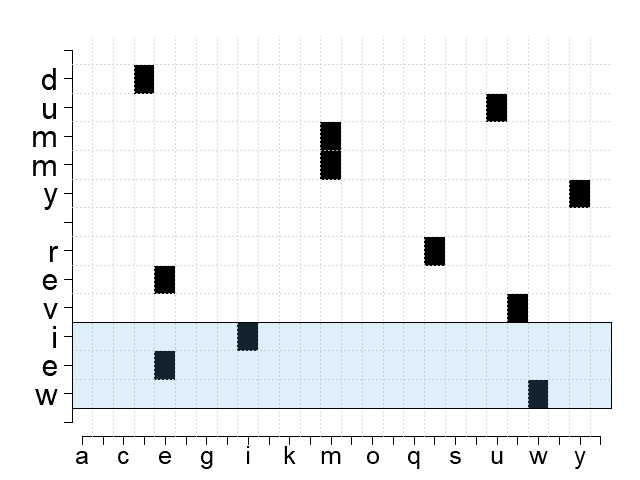
\includegraphics[width=9cm]{figure/11_encoded_text.png}}%
    \\
    \begin{itemize}
        \only<1>{\item We encode text on a character level (here: \textit{\enquote{dummy review}}). Each character becomes a one-hot vector over the alphabet.}
        \only<1>{\item Reviews are padded or truncated to a fixed length (e.g.\ 1014 characters).}
        \only<2>{\item The result is a 1D signal with \emph{depth = alphabet size}.}
        \only<3>{\item The temporal dimension is shown on the $y$-axis for illustration.}
        \only<4>{\item The 1D kernel (blue) convolves along the temporal dimension, yielding a 1D feature vector.}
    \end{itemize}
}
%%%%%%%%%%%%%%%%%%%%%%%%%%%%%%%%%%%%%%%%%%%%%%%%

\begin{vbframe}{Advantages of 1D Convolutions}
For certain applications, 1D CNNs are preferable to their 2D counterparts:
   \begin{itemize}
     \item \textbf{Computational complexity}: forward and backward passes reduce to simple array operations.
     \item \textbf{Training}: shallow 1D architectures are often sufficient for challenging 1D-signal tasks.
     \item \textbf{Hardware}: deep 2D CNNs usually need specialized hardware, while compact 1D CNNs train well on a standard CPU.
     \item \textbf{Application}: low computational cost makes compact 1D CNNs well suited to real-time and low-cost applications, e.g.\ on mobile or embedded devices.
     \end{itemize}
\end{vbframe}

%%%%%%%%%%%%%%%%%%%%%%%%%%%%%%%%%%%%%%%%%%%%%%%
\section{2D Convolutions}
%%%%%%%%%%%%%%%%%%%%%%%%%%%%%%%%%%%%%%%%%%

\begin{vbframe}{2D Convolutions}
The basic idea behind a 2D convolution is sliding a small window (the ``kernel''/``filter'') over a larger 2D array, computing a dot product between the filter and the corresponding input elements at every position.
    \begin{figure}
        \centering
        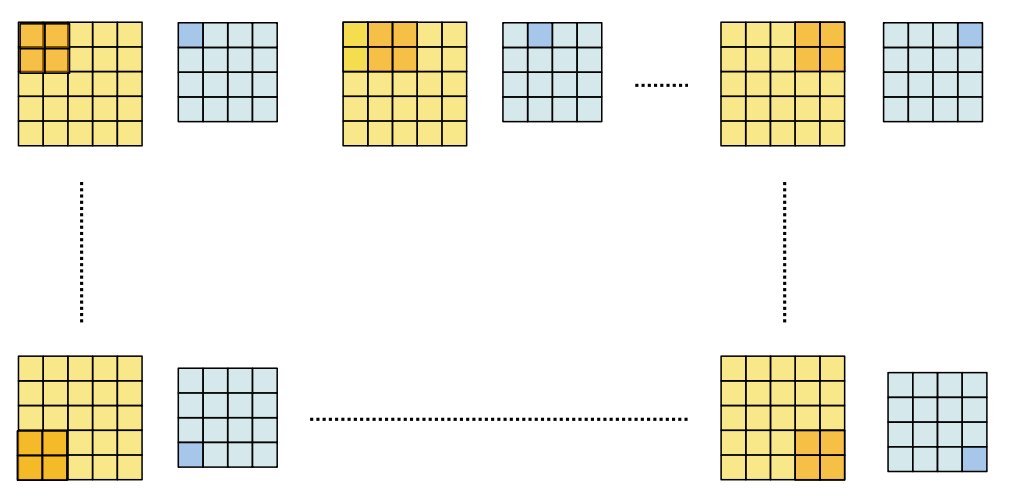
\includegraphics[width=9cm]{figure/padding3.png}
        \caption{\tiny Applying a $2\times 2$ convolution filter to a $5\times 5$ array, at 16 different positions.}
    \end{figure}
\end{vbframe}
%%%%%%%%%%%%%%%%%%%%%%%%%%%%%%%%%%%%%%%%%%%%%%

\frame{
\frametitle{2D Convolutions --- Example}
    \center
    \only<1>{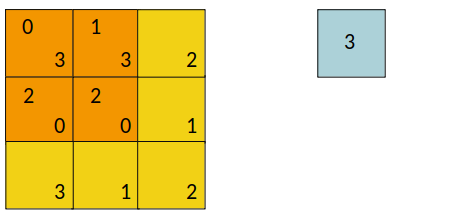
\includegraphics[width=9cm]{figure/conv2d-1.png}}%
    \only<2>{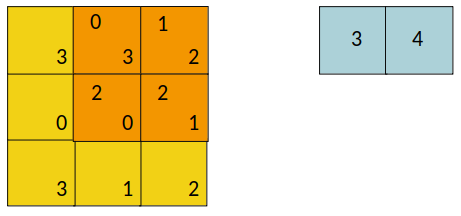
\includegraphics[width=9cm]{figure/conv2d-2.png}}%
    \only<3>{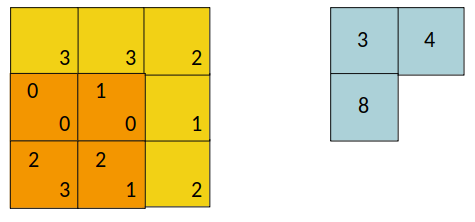
\includegraphics[width=9cm]{figure/conv2d-3.png}}%
    \only<4>{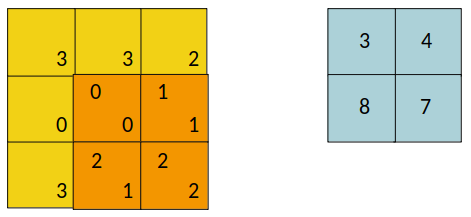
\includegraphics[width=9cm]{figure/conv2d-4.png}}%
    \begin{itemize}
        \only<1>{\item In deep learning, convolution means element-wise multiplication followed by addition. For a single-channel image with a $2\times 2$ filter $[[0,1],[2,2]]$: }
        \only<2>{\item The filter slides through the input, computing a new feature map.}
        \only<3>{\item Notice: stride is 1 and padding is 0 in this example.}
        \only<4>{\item Each sliding position yields one number; the output here is a $2\times 2$ matrix.}
    \end{itemize}
}

%%%%%%%%%%%%%%%%%%%%%%%%%%%%%%%%%%%%%%%%%%%%%%%%%%%%

\section{3D Convolutions}

\begin{vbframe}{3D Convolutions}
\textbf{Data situation}: 3-dimensional tensor data.
    \begin{itemize}
        \item Data consists of tensors with shape [depth, xdim, ydim, zdim].
        \item Dimensions can be temporal (e.g.\ video frames) or spatial (e.g.\ MRI).
        \item Examples: human activity recognition in video, disease classification or tumor segmentation on MRI scans.
    \end{itemize}
\textbf{Solution}: move a 3D kernel in $x$, $y$, and $z$ direction to capture all relevant information.
\end{vbframe}
%%%%%%%%%%%%%%%%%%%%%%%%%%%%%%%%%%%%%%%%%%%%%%%%
\begin{frame}{3D Convolutions --- Data}
    \begin{figure}
        \centering
        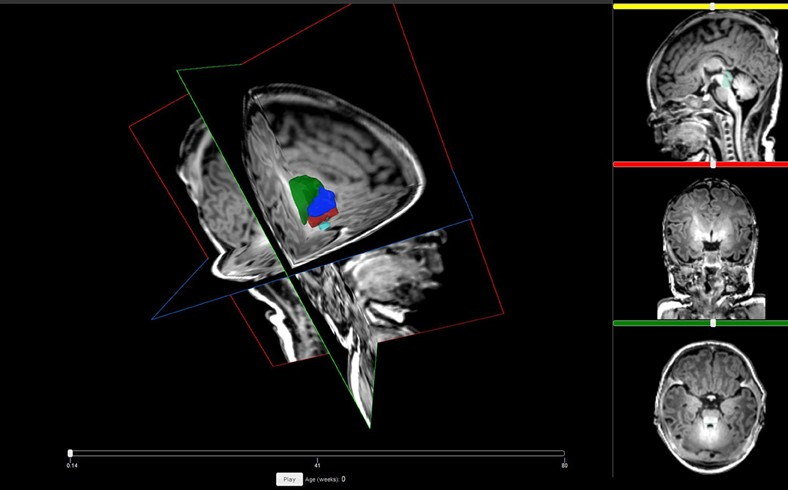
\includegraphics[width=5cm]{figure/mri.jpg}
        \caption{Depth-$1$ volumetric data: an MRI scan. Each slice has depth $1$, as the frames are black-and-white (Gutman et al., 2014).}
    \end{figure}
\end{frame}
%%%%%%%%%%%%%%%%%%%%%%%%%%%%%%%%%%%%%%%%%%%%%%%%%

\begin{frame}{3D Convolutions --- Data}
    \begin{figure}
        \centering
        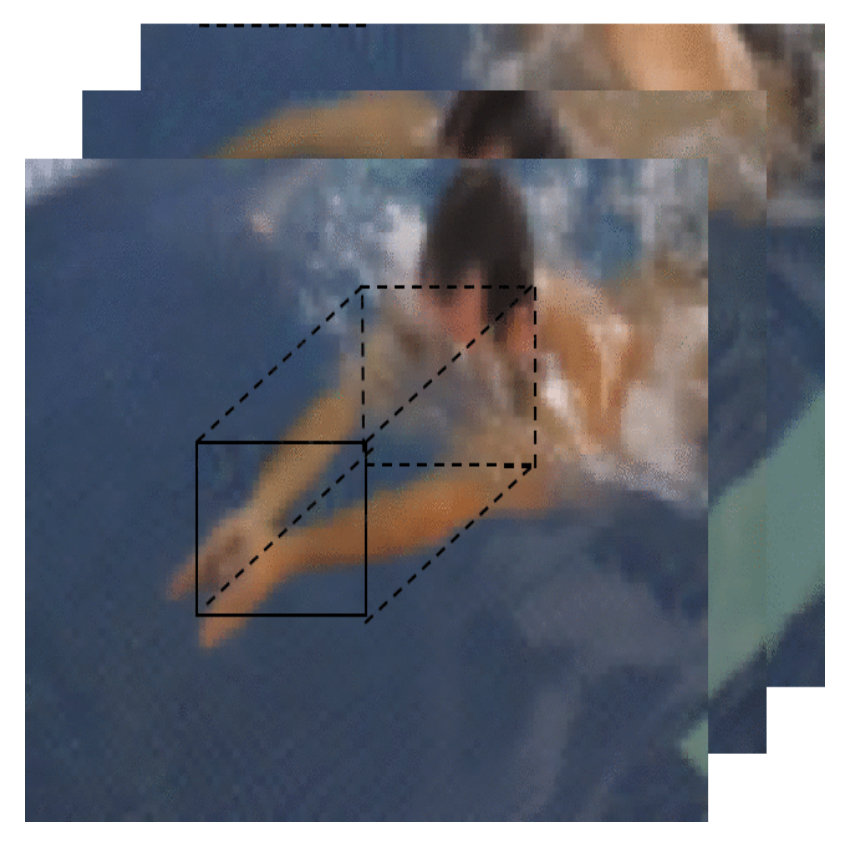
\includegraphics[width=5cm]{figure/swim.png}
        \caption{Volumetric data with depth $>1$: a video snippet for action detection. The video is several RGB (depth-$3$) slices stacked in temporal order (Ghosh, 2018).}
    \end{figure}
\end{frame}
%%%%%%%%%%%%%%%%%%%%%%%%%%%%%%%%%%%%%%%%%%%%%%%%%

\begin{vbframe}{3D Convolutions --- Architecture}
    \begin{figure}
        \centering
        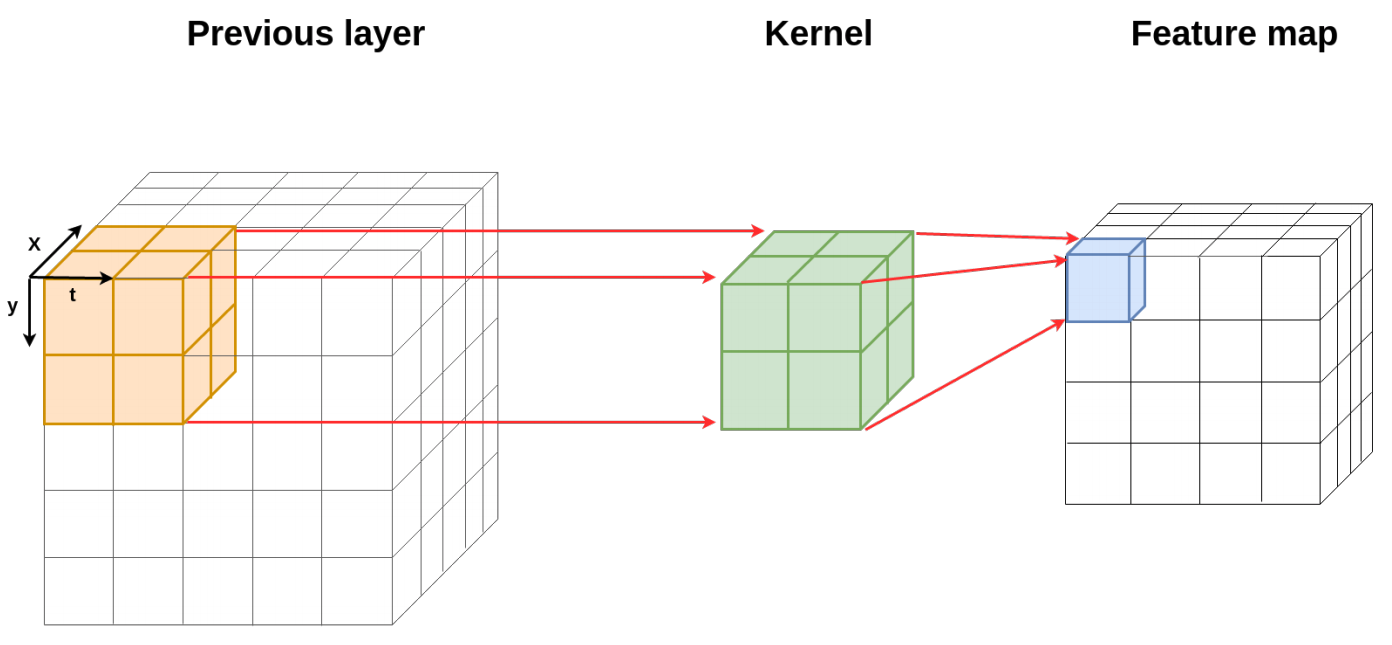
\includegraphics[width=8cm]{figure/3dconv.png}
        \caption{3D convolutions yield a 3D output.}
    \end{figure}
    \begin{figure}
        \centering
        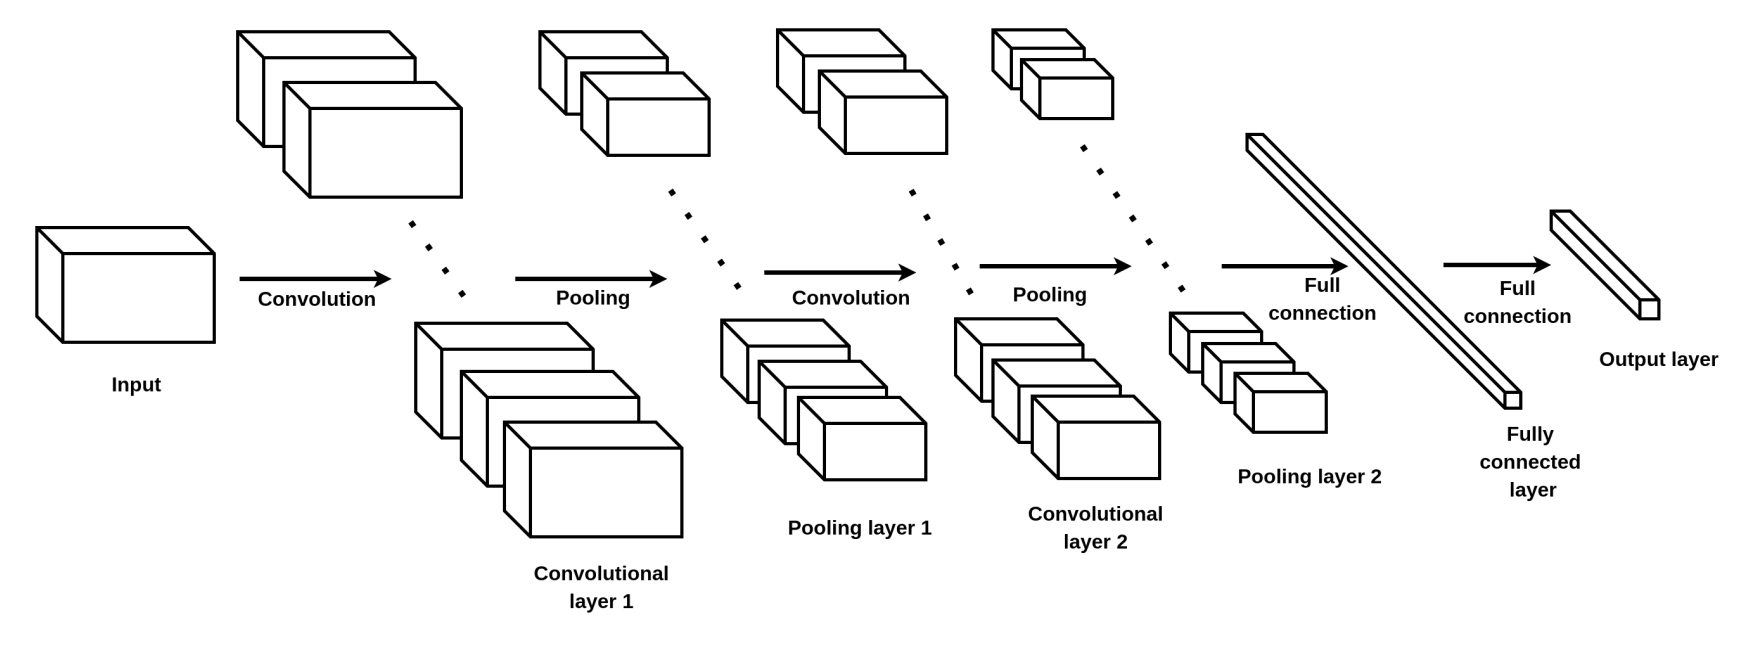
\includegraphics[width=11cm]{figure/3dconv_arch.png}
        \caption{A basic 3D-CNN architecture: the overall structure is unchanged, but feature maps are now 3D, element-wise activated, and (eventually) pooled in 3 dimensions.}
    \end{figure}
\end{vbframe}
%%%%%%%%%%%%%%%%%%%%%%%%%%%%%%%%%%%%%%%%%%%%%
%%%%%%%%%%%%%%%%%%          REFERENCES          %%%%%%%%%%%%%%%%%%
%%%%%%%%%%%%%%%%%%%%%%%%%%%%%%%%%%%%%%%%%%%%%%%%%%%%%%%%%%%%%%%%%%
\begin{vbframe}
\frametitle{References}
\footnotesize{
\begin{thebibliography}{99}
\bibitem[(Ismail Fawaz et al., 2019)]{1} Ismail Fawaz, H., Forestier, G., Weber, J., Idoumghar, L., \& Muller, P.-A. (2019). Deep learning for time series classification: a review. \textit{Data Mining and Knowledge Discovery}, 33. \url{https://doi.org/10.1007/s10618-019-00619-1}
\bibitem[(Gutman et al., 2014)]{2} Gutman, D., Dunn Jr, W., Cobb, J., Stoner, R., Kalpathy-Cramer, J., \& Erickson, B. (2014). Web based tools for visualizing imaging data and development of XNATView, a zero footprint image viewer. \textit{Frontiers in Neuroinformatics}, 8, 53. \url{https://doi.org/10.3389/fninf.2014.00053}
\bibitem[(Ghosh, 2018)]{3} Ghosh, R. (2018, June 11). \textit{Deep learning for videos: A 2018 guide to action recognition}. \url{https://blog.qure.ai/notes/deep-learning-for-videos-action-recognition-review}
\end{thebibliography}
}
\end{vbframe}

%%%%%%%%%%%%%%%%%%%%%%%%%%%%%%%%%%%%%%%%%%%%%%%%%%%%%%%%%%%%%%%%%%
\section{CNN Components: Channels, Padding, Stride}
%%%%%%%%%%%%%%%%%%%%%%%%%%%%%%%%%%%%%%%%%%%%%%%%%%%%%%%%%%%%%%%%%%

\begin{vbframe}{Input Channels}
         \begin{figure}
    \centering
    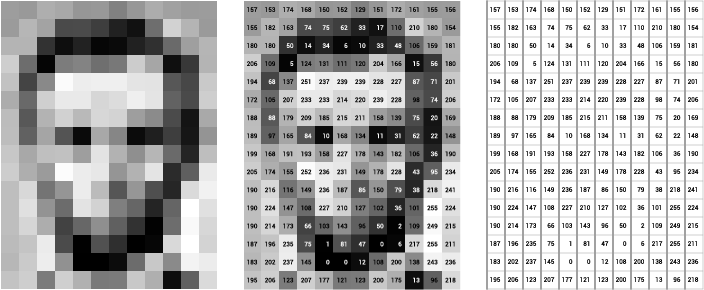
\includegraphics[width=4cm]{figure/gray.png}
        \caption{Left: image of Lincoln; center: pixels labeled with grayscale values; right: grayscale values alone (Levin \& Dorsey).}
  \end{figure}
    \begin{itemize}
       \item An image consists of the smallest indivisible segments, called pixels, each with an intensity value.
       \item A grayscale image has a single input channel, with each pixel's value representing brightness.
       \item Grayscale values range from 0 to 255 (0 = black, 255 = white).
    \end{itemize}
\end{vbframe}

\begin{vbframe}{Input Channels --- Color}
 \begin{figure}
    \centering
    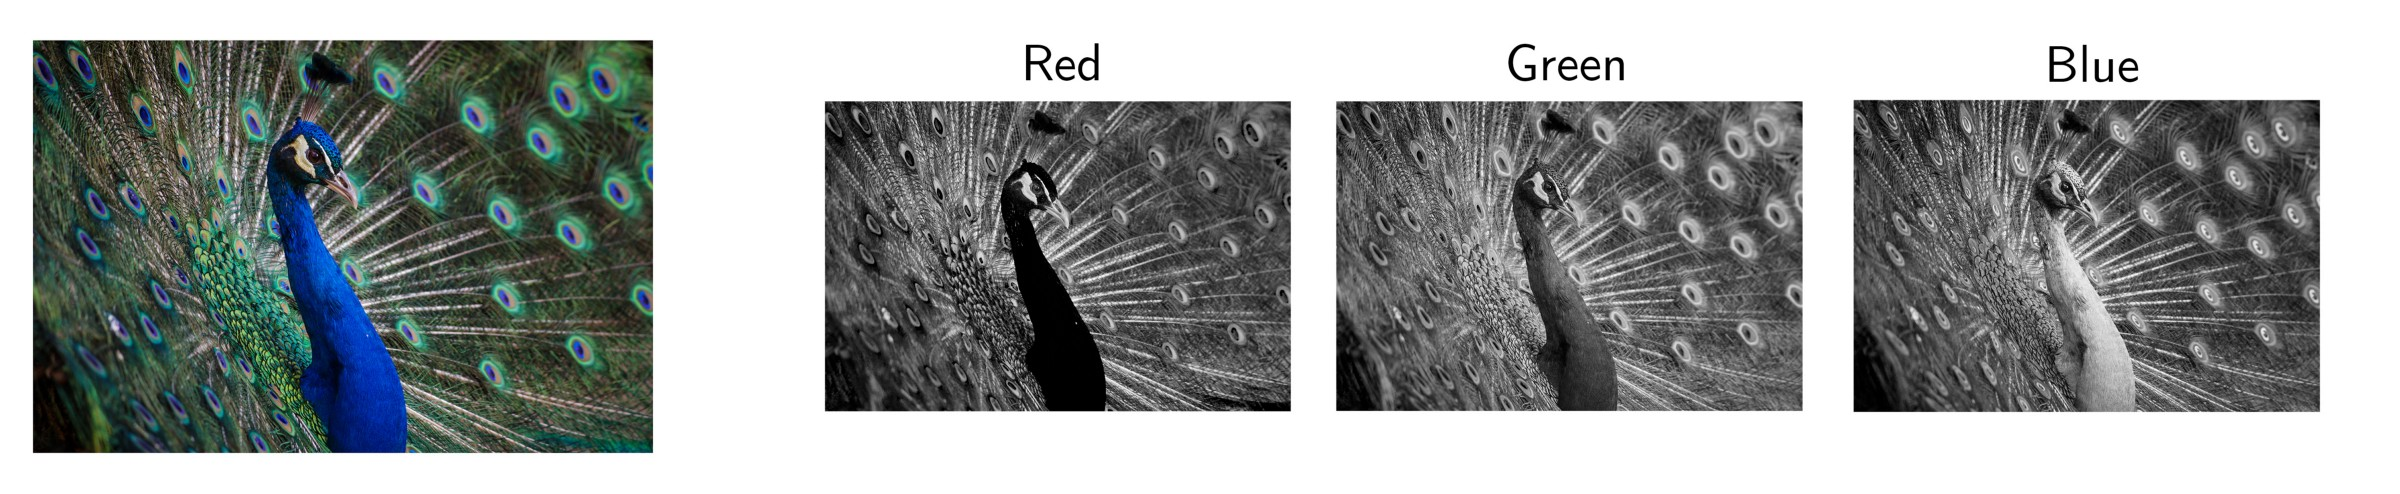
\includegraphics[width=7cm]{figure/RGB.jpeg}
  \end{figure}
 \begin{figure}
    \centering
    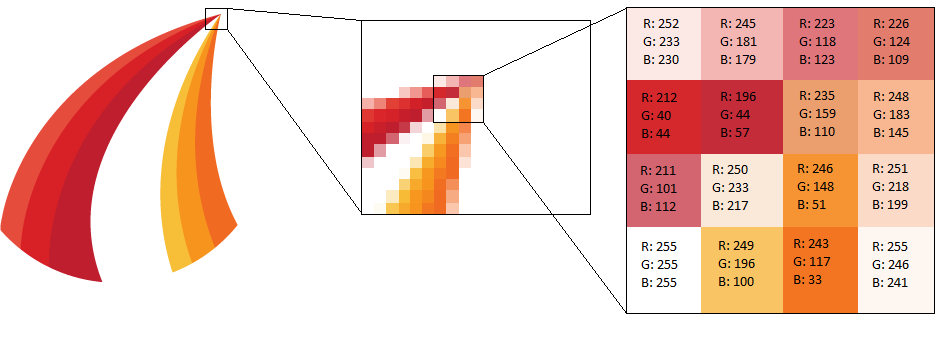
\includegraphics[width=5cm]{figure/RGB-1.png}
    \caption{How a CNN ``sees'' an image (Maladkar, 2020).}
  \end{figure}
\begin{itemize}
       \item A color digital image usually has three color channels --- Red, Green, Blue (RGB).
        \item Each pixel is a vector of three numbers (each in $[0,255]$), one per color channel.
\end{itemize}
\end{vbframe}

%%%%%%%%%%%%%%%%%%%%%%%%%%%%%%%%%%%%%%%%%%%%%%%%%%%%%%%%%%%%%%%55%%

\begin{frame}{Valid Padding}
\begin{itemize}
\only<1>{\item[] Suppose we have an input of size $5 \times 5$ and a filter of size $2 \times 2$.}
\only<2>{\item[] The filter is only allowed to move inside the input space.}
\only<3>{\item[] That inevitably reduces the output dimensions.}
\end{itemize}
\center
\only<1>{\scalebox{0.5}{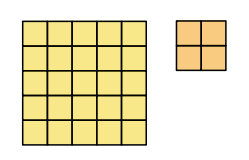
\includegraphics{figure/padding1.png}}}%
\only<2>{\scalebox{0.5}{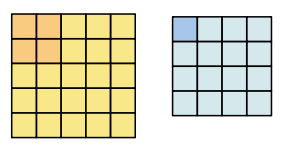
\includegraphics{figure/padding2.png}}}%
\only<3>{\scalebox{1}{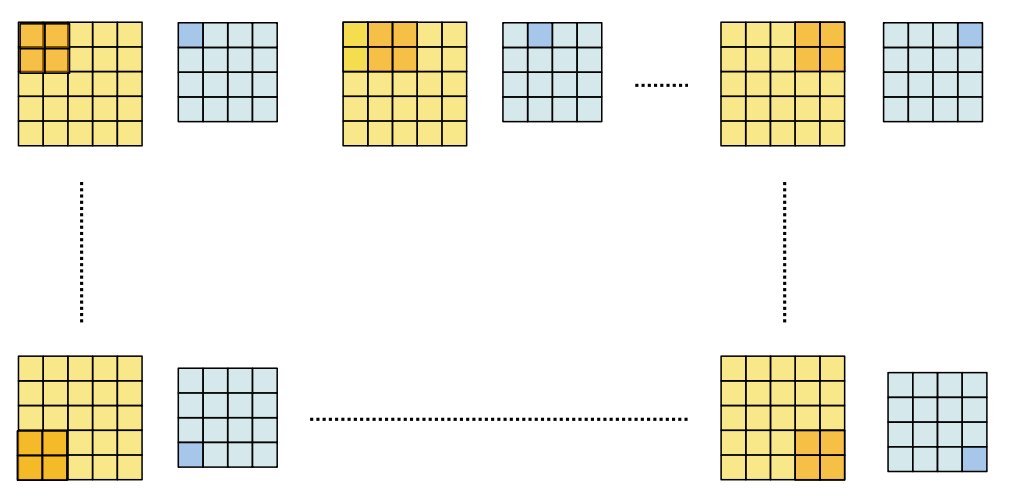
\includegraphics{figure/padding3.png}}}%
\only<3>{\item[] In general, for an input of size $i\, (\times\, i)$ and filter size $k\, (\times\, k)$, the output feature map size $o\, (\times\, o)$ is:
    $$ o =  i-k + 1 $$ }
\end{frame}
%%%%%%%%%%%%%%%%%%%%%%%%%%%%%%%%%%%%%%%%%%%%%%%%%%%%%%%%%%%%%%%%%%

\begin{frame}{Same Padding}
\begin{itemize}
\only<1>{\item[] Suppose an input of dimensions $5 \times 5$ and a filter of size $3 \times 3$.}
\only<2>{\item[] We want an output with the \emph{same} dimensions as the input.}
\only<3>{\item[] Solution: zero padding --- pad zeros around the input.}
\only<4>{\item[] This always works: we just adjust the amount of padding to the input dimensions and filter size.}
  \end{itemize}
  \center
  \only<1>{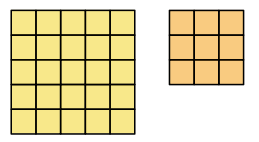
\includegraphics[width=5cm]{figure/padding4.png}}%
  \only<2>{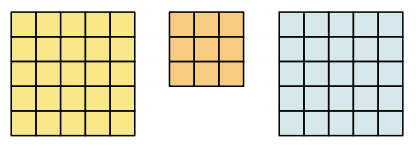
\includegraphics[width=8cm]{figure/padding5.png}}%
  \only<3>{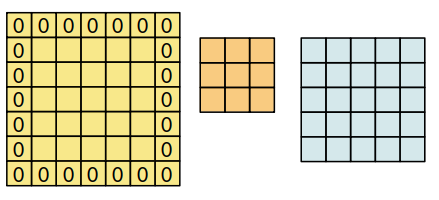
\includegraphics[width=8cm]{figure/padding6.png}}%
  \only<4>{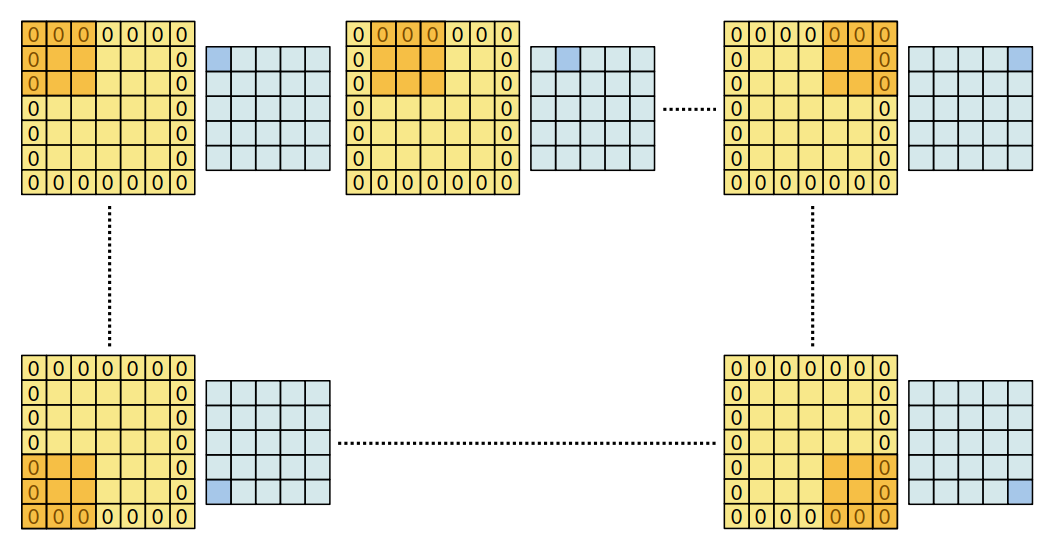
\includegraphics[width=11cm]{figure/padding7.png}}%
\end{frame}
%%%%%%%%%%%%%%%%%%%%%%%%%%%%%%%%%%%%%%%%%%%%%%%%%%%%%%%%%%%%%%%%%%

\begin{frame}{Padding and Network Depth}
\begin{figure}
\center
\scalebox{0.4}{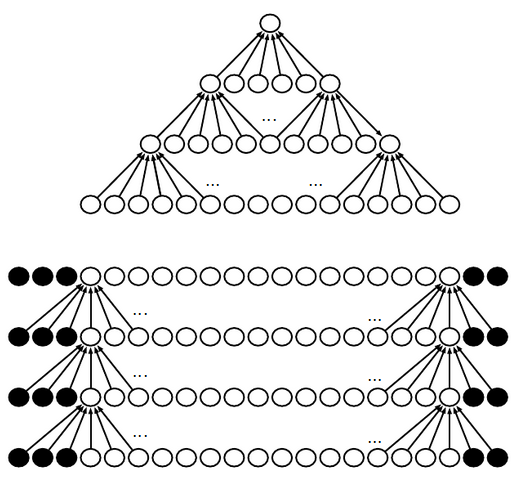
\includegraphics{figure/zeropadding.png}}
\caption{\small{\enquote{Valid} vs.\ \enquote{same} convolution.
\\ \emph{Top}: without padding, the feature map width shrinks rapidly (to 1 after just three layers here), limiting network depth.
\\ \emph{Bottom}: with zero padding, the feature map stays the same size after each convolution, so the network can be made arbitrarily deep (Goodfellow et al., 2016).}}
\end{figure}
\end{frame}
%%%%%%%%%%%%%%%%%%%%%%%%%%%%%%%%%%%%%%%%%%%%%%%%%%%%%%%%%%%%%%%%%%
\section{Stride}
%%%%%%%%%%%%%%%%%%%%%%%%%%%%%%%%%%%%%%%%%%%%%%%%%%%%%%%%%%%%%%%%%%

\frame{
\frametitle{Strides}
  \begin{itemize}
    \only<1-3>{\item The step size (\enquote{stride}) with which the filter moves (stride = 2 shown below).}
  \end{itemize}
  \center
  \only<1>{\scalebox{0.4}{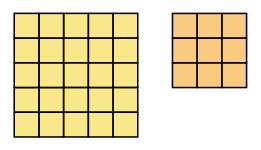
\includegraphics{figure/stride1.png}}}%
  \only<2>{\scalebox{0.35}{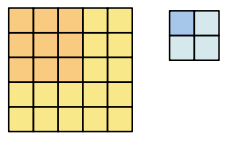
\includegraphics{figure/stride2.png}}}%
  \only<3>{\scalebox{0.7}{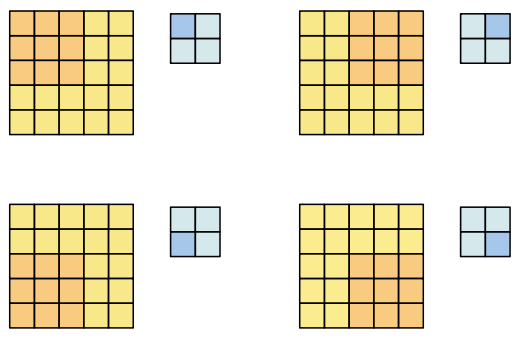
\includegraphics[width=9cm]{figure/stride3.png}}}%
  \only<3>{\item[] In general, with no padding, for input size $i$, filter size $k$, and stride $s$, the output size $o$ is:
    $$ o=\left\lfloor\frac{i-k}{s}\right\rfloor+ 1 $$ }
}

\frame{
\frametitle{Strides and Downsampling}
\begin{figure}
\center
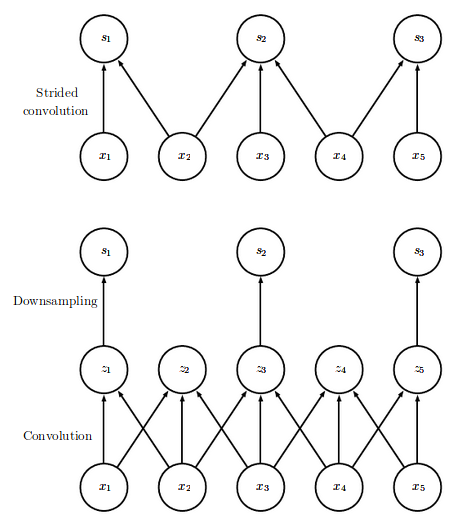
\includegraphics[width=.5\textwidth]{figure/stride4.png}
\caption{A strided convolution is equivalent to a convolution without stride, followed by downsampling (Goodfellow et al., 2016).}
\end{figure}
}
%%%%%%%%%%%%%%%%%%%%%%%%%%%%%%%%%%%%%%%%%%%%%%%%%%%%%%%%%%%%%%%%%%

\begin{vbframe}{Putting It Together}
 \begin{figure}
    \centering
    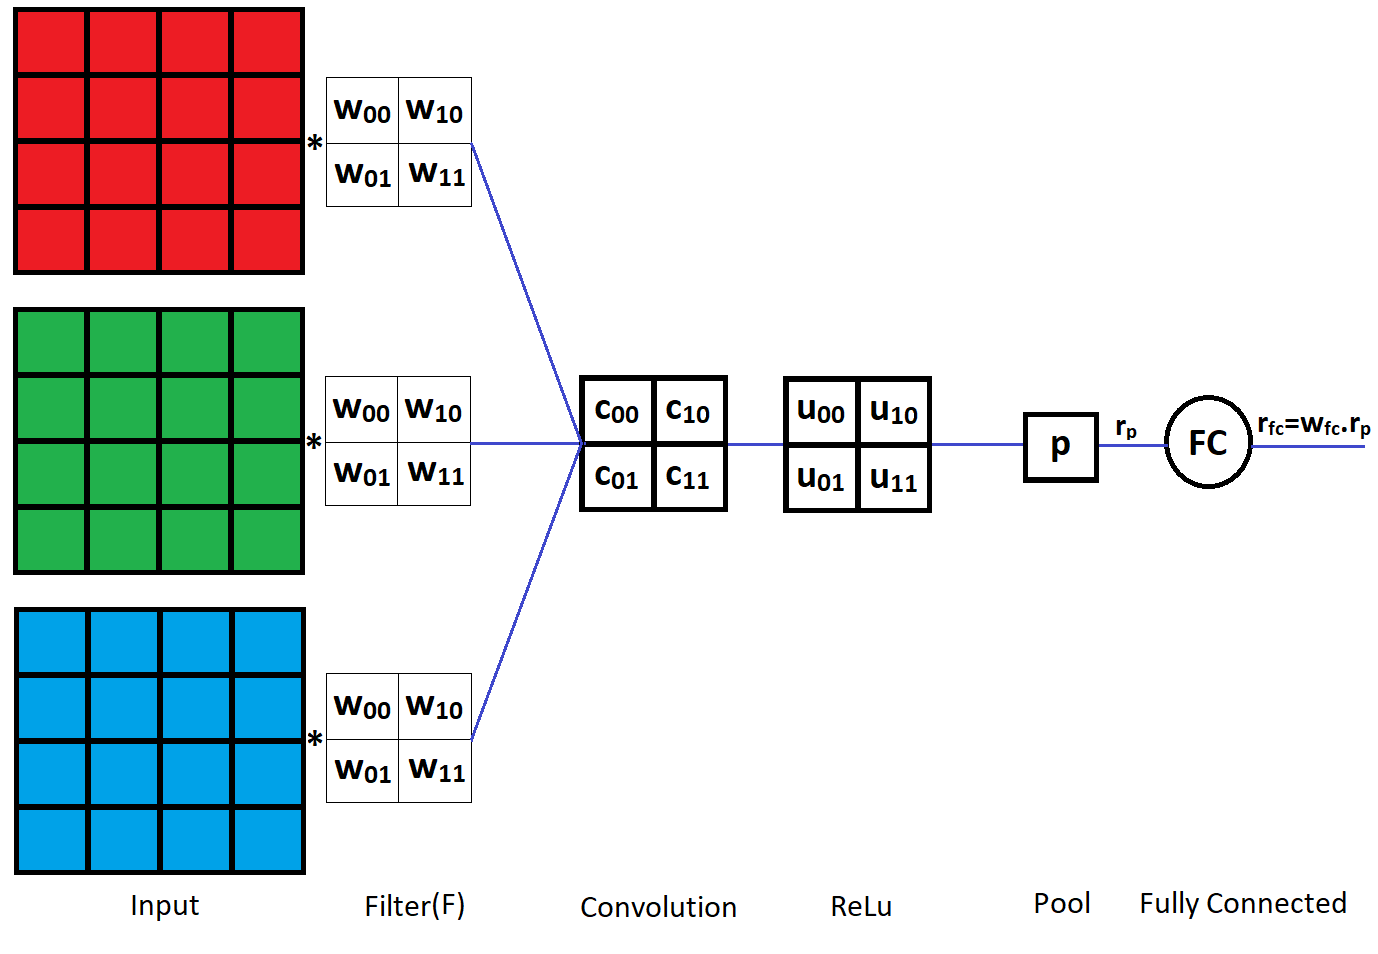
\includegraphics[width=5cm]{figure/3channel.png}
    \caption{For color images, Red, Green, and Blue each serve as a separate input channel (Belwal, 2018).}
  \end{figure}
This CNN has:
    \begin{itemize}
       \item 3 input channels, with a $4\times 4$ input matrix each,
       \item one $2\times 2$ filter (kernel),
       \item a single ReLU layer,
       \item a single max-pooling layer,
       \item and a single fully connected (FC) layer.
    \end{itemize}
    \begin{itemize}
       \item The filter entries are equivalent to unit weights in a standard NN, updated during backpropagation.
       \item With stride 2 and no padding, the output size of the convolution layer is:
       \item $ o = \frac{i - k + 2p}{s} + 1$, where $i$ = input size, $k$ = filter size, $p$ = padding, $s$ = stride.
    \end{itemize}
Inserting the figure's values:
\begin{align}
o= \frac{i - k + 2p}{s} + 1&={(4 - 2 + 2 \cdot 0)\over 2} + 1\\
&=2
\end{align}
\end{vbframe}
%%%%%%%%%%%%%%%%%%%%%%%%%%%%%%%%%%%%%%%%%%%%%%%%%%%%%%%%%%%%%%%%%%
%%%%%%%%%%%%%%%%%%          REFERENCES          %%%%%%%%%%%%%%%%%%
%%%%%%%%%%%%%%%%%%%%%%%%%%%%%%%%%%%%%%%%%%%%%%%%%%%%%%%%%%%%%%%%%%
\begin{vbframe}
\frametitle{References}
\footnotesize{
\begin{thebibliography}{99}
\bibitem[(Levin \& Dorsey)]{1} Levin, G. (n.d.). \textit{Image Processing and Computer Vision}. ofBook. \url{https://openframeworks.cc/ofBook/chapters/image_processing_computer_vision.html}
\bibitem[(Goodfellow et al., 2016)]{2} Goodfellow, I., Bengio, Y., \& Courville, A. (2016). \textit{Deep Learning}. MIT Press.
\bibitem[(Belwal, 2018)]{3} Belwal, C. (2018, June 12). \textit{Part III: Backpropagation mechanics for a convolutional neural network}. \url{http://cbelwal.blogspot.com/2018/05/part-iii-backpropagation-mechanics-for.html}
\bibitem[(Maladkar, 2020)]{4} Maladkar, K. (2020, October 16). \textit{Computer vision primer: How AI sees an image}. Analytics India Magazine. \url{https://analyticsindiamag.com/computer-vision-primer-how-ai-sees-an-image/}
\end{thebibliography}
}
\end{vbframe}

%%%%%%%%%%%%%%%%%%%%%%%%%%%%%%%%%%%%%%%%%%%%%%%%%%%%%%%%%%%%%%%%%%
\section{Properties of Convolution}
%%%%%%%%%%%%%%%%%%%%%%%%%%%%%%%%%%%%%%%%%%%%%%%%%%%%%%%%%%%%%%%%%%

\begin{vbframe}{Sparse Interactions and Parameter Sharing}
  \begin{itemize}
    \item Unlike a dense layer, a convolutional layer connects each output unit only to a small, local \textbf{receptive field} of the input --- a \enquote{local search} for features, instead of a dense layer's \enquote{global search}.
    \item The same filter weights are reused (\textbf{shared}) at every spatial location, instead of learning a separate weight per input--output pair.
    \item Why this matters: for $m$ inputs and $n$ outputs, a dense layer needs $\mathcal{O}(m \times n)$ parameters and runtime; a convolutional layer with a local filter of size $k \ll m$ needs only $\mathcal{O}(k \times n)$ --- drastically less memory, faster runtime, and typically less overfitting.
    \item Example: a $100\times 100$ color image, one same-padded feature map, filter size $5$: a conv layer uses $5\cdot 5\cdot 3 = 75$ parameters; a dense layer with the same number of hidden units uses $100^2 \cdot 3 \cdot 100^2 = 300{,}000{,}000$.
  \end{itemize}
\end{vbframe}
%%%%%%%%%%%%%%%%%%%%%%%%%%%%%%%%%%%%%%%%%%%%%%%%%%%%%%%%%%%%%%%%%%

\frame{
\frametitle{Equivariance to Translation}
  \center
  \only<1>{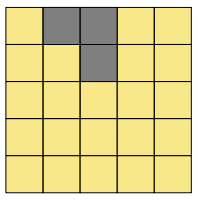
\includegraphics[width=5cm]{figure/equivariance1.png}}%
  \only<2>{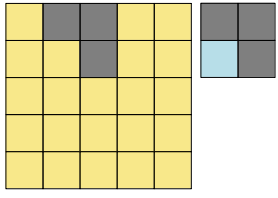
\includegraphics[width=7cm]{figure/equivariance2.png}}%
  \only<3>{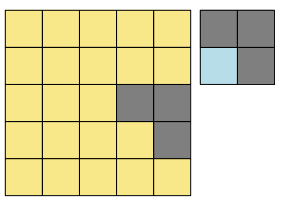
\includegraphics[width=7cm]{figure/equivariance3.png}}%
  \only<4>{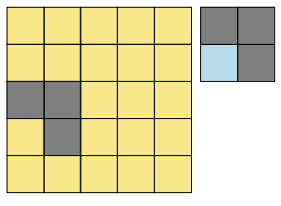
\includegraphics[width=7cm]{figure/equivariance4.png}}%
  \begin{itemize}
    \only<1>{\item Think of a specific feature of interest, highlighted in grey.}
    \only<2>{\item Assume we have a filter tuned to look for exactly that feature.}
    \only<3>{\item The filter does not care \emph{where} the feature is located.}
    \only<4>{\item It can find it anywhere --- this property is called \textbf{equivariance to translation}. \\[0.2cm] \scriptsize{A function $f$ is equivariant to a function $g$ if $f(g(x)) = g(f(x))$.}}
  \end{itemize}
}
%%%%%%%%%%%%%%%%%%%%%%%%%%%%%%%%%%%%%%%%%%%%%%%%%%%%%%%%%%%%%%%%%%

\begin{frame}{Nonlinearity in Feature Maps}
    \begin{itemize}
        \item As in dense nets, we apply an activation function to every feature-map entry to introduce nonlinearity.
        \item Typically ReLU (or a variant: Leaky ReLU, ELU, PReLU, \ldots, covered in Session 2) is used:
            \begin{itemize}
                \item reduces the risk of saturating gradients compared to sigmoid activations,
                \item can lead to \textit{sparse activations} (entries $\le 0$ are squashed to $0$), which speeds up computation.
            \end{itemize}
    \end{itemize}
\end{frame}

%%%%%%%%%%%%%%%%%%%%%%%%%%%%%%%%%%%%%%%%%%%%%%%%%%%%%%%%%%%%%%%%%%
\section{Dilated and Transposed Convolutions}
%%%%%%%%%%%%%%%%%%%%%%%%%%%%%%%%%%%%%%%%%%%%%%%%%%%%%%%%%%%%%%%%%%

\begin{frame}{Dilated Convolutions}
    \begin{itemize}
        \item Idea: artificially increase the net's receptive field without adding more filter weights.
        \item The \textbf{receptive field} of a neuron comprises all inputs that affect it. Neurons in early layers capture little of the input; neurons in later layers have huge receptive fields and capture much more global information. Receptive-field size depends on filter size.
    \end{itemize}
    \vspace*{-0.5cm}
    \begin{figure}
        \centering
        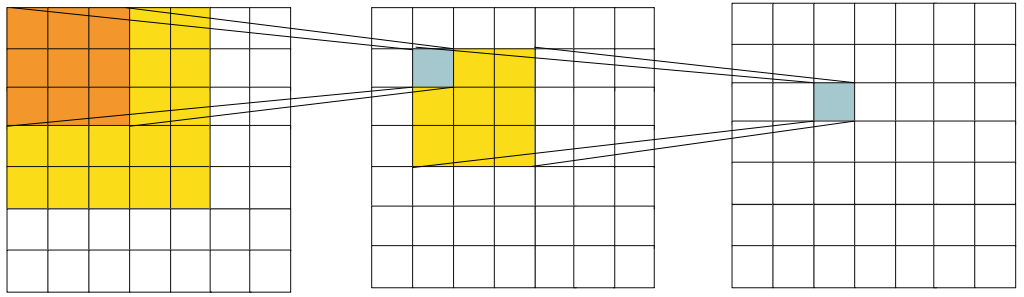
\includegraphics[width=7cm]{figure/dilatedconv-6.png}
        \caption{Receptive field of each layer with a $3\times 3$ kernel. Orange marks the receptive field of one pixel in Layer 2, yellow the receptive field of one pixel in Layer 3.}
    \end{figure}
\end{frame}
%%%%%%%%%%%%%%%%%%%%%%%%%%%%%%%%%%%%%%%%%%%%

\begin{frame}{Dilated Convolutions}
\begin{itemize}
        \item Increasing filter size grows the receptive field and captures more context, but also increases the number of parameters and runtime.
        \item Instead: add a \textbf{dilation} parameter that skips pixels during convolution, artificially increasing the receptive field without more weights.
        \item Benefits: more contextual information, higher-dimensional inputs stay tractable, better runtime (fewer parameters).
        \item Useful wherever global context matters for the decision --- e.g.\ WaveNet's audio generation, time-series classification/forecasting, image segmentation.
    \end{itemize}
    \begin{figure}
        \centering
        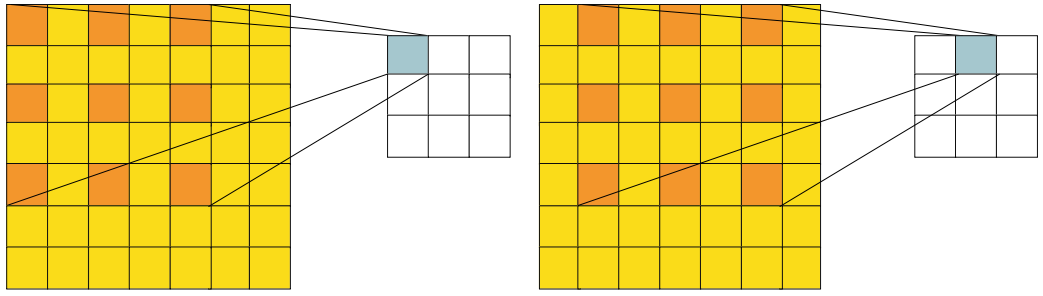
\includegraphics[width=7cm]{figure/dilatedconv-7.png}
        \caption{Dilated convolution on 2D data: a dilated kernel is a regular kernel interleaved with zeros.}
    \end{figure}
\end{frame}
%%%%%%%%%%%%%%%%%%%%%%%%%%%%%%%%%%%%%%%%%%%%

\begin{frame}{Dilated Convolutions}
    \vspace*{0.5cm}
    \begin{figure}
        \centering
        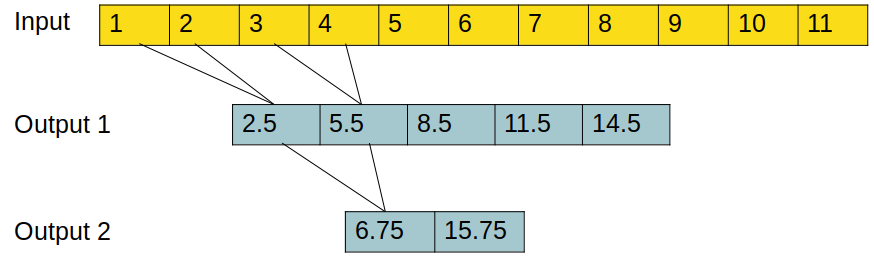
\includegraphics[width=11cm]{figure/dilatedconv-4.png}
        \caption{1D conv, kernel size $2$, stride $2$, weights $\{0.5, 1.0\}$, \textbf{dilation factor 1}: one neuron in layer 2 has receptive field $4$.}
    \end{figure}
\end{frame}
%%%%%%%%%%%%%%%%%%%%%%%%%%%%%%%%%%%%%%%%%%%%

\begin{frame}{Dilated Convolutions}
    \vspace*{0.5cm}
    \begin{figure}
        \centering
        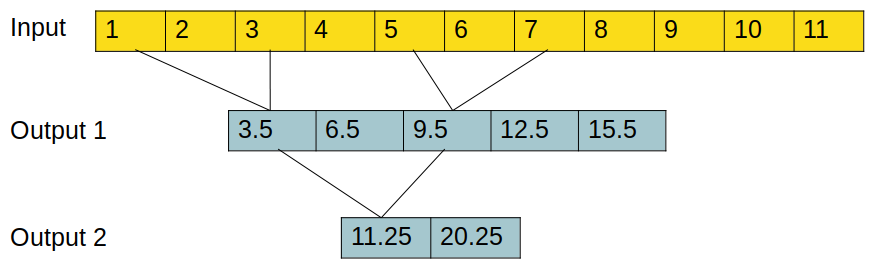
\includegraphics[width=11cm]{figure/dilatedconv-5.png}
        \caption{Same setup with \textbf{dilation factor 2}: one neuron in layer 2 now has receptive field $7$.}
    \end{figure}
\end{frame}
%%%%%%%%%%%%%%%%%%%%%%%%%%%%%%%%%%%%%%%%%%%%

\begin{frame}{Dilated Convolutions}
    \begin{figure}
        \centering
        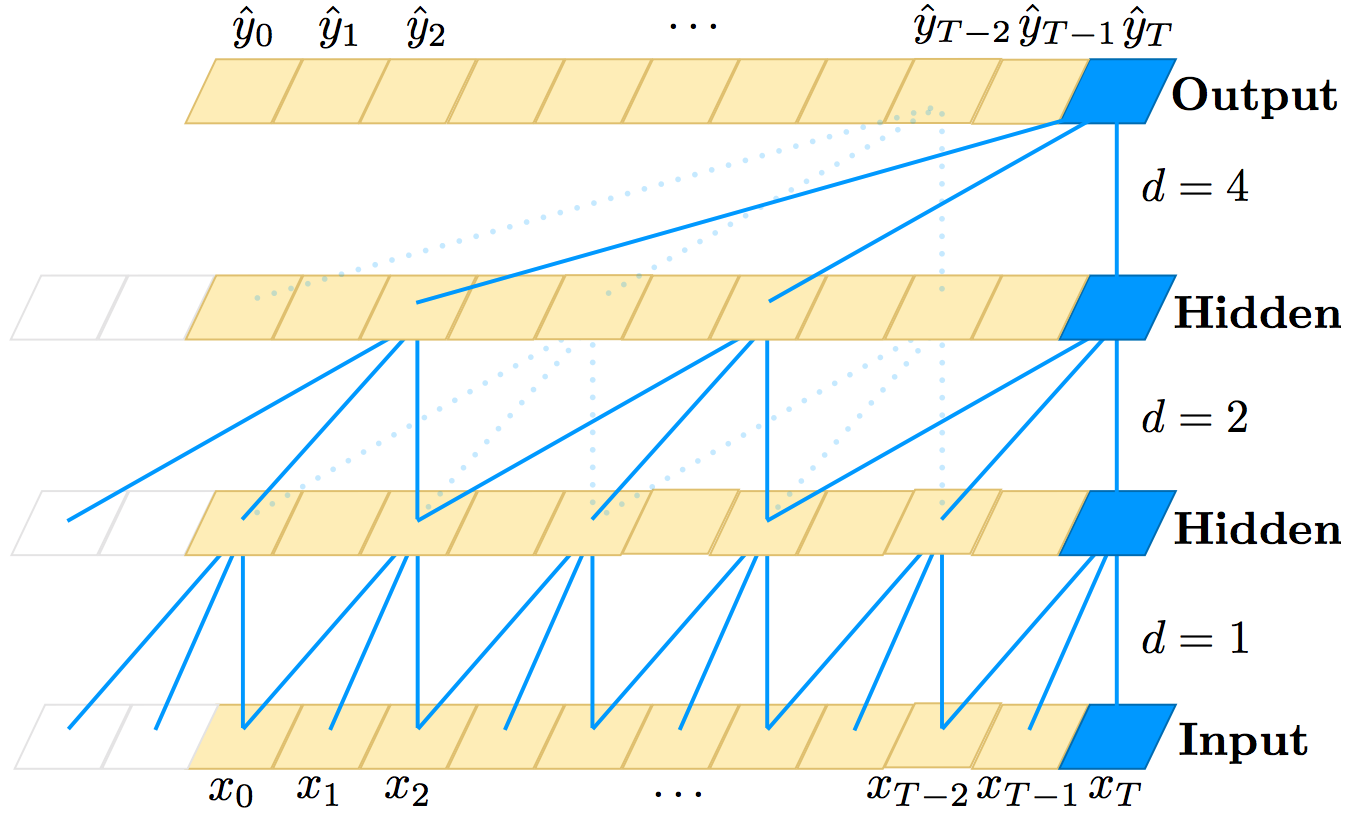
\includegraphics[width=8cm]{figure/tcn.png}
        \caption{Dilated convolutions on a time series for classification or seq2seq prediction. Given $x_0,\ldots,x_T$, the model outputs $\yh_0,\ldots,\yh_T$. Dilation factors $d=1,2,4$ with kernel size $k=3$ drastically increase context per output neuron with few layers (Roy, 2019).}
    \end{figure}
\end{frame}
%%%%%%%%%%%%%%%%%%%%%%%%%%%%%%%%%%%%%%%%%%%%

\begin{vbframe}{Transposed Convolutions}
    \begin{itemize}
        \item Problem setting: many architectures need to go in the \emph{opposite} direction of a regular convolution, i.e.\ upsampling --- e.g.\ generating high-resolution images, or mapping a low-dimensional feature map to a high-dimensional space (autoencoders, semantic segmentation).
        \item Instead of decreasing dimensionality, \textbf{transposed convolutions} re-increase it.
        \item Note: not the same as \emph{deconvolution} (the mathematical inverse of a convolution).
    \end{itemize}
\framebreak
\begin{itemize}
\item Example: input $4\times 4$ (yellow), output $2\times 2$ (blue).
\end{itemize}
\begin{figure}
\centering
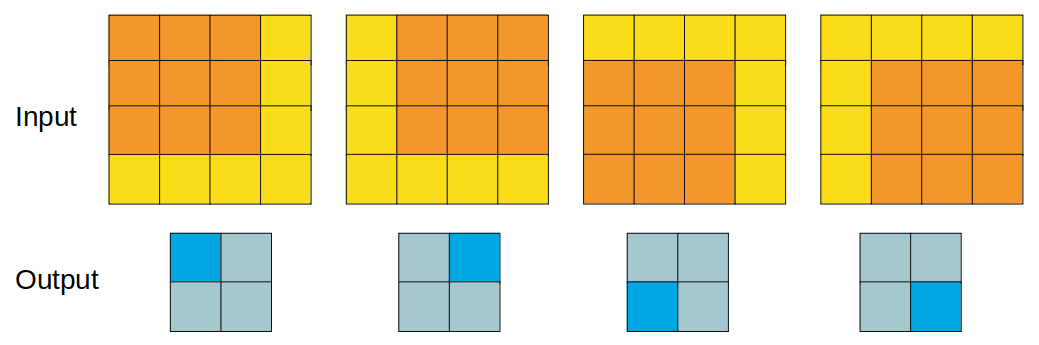
\includegraphics[width=10cm]{figure/transposedconv-1.png}
      \caption{A \textbf{regular} convolution, $k=3$, $p=0$, $s=1$: the feature map shrinks from $4\times 4$ to $2\times 2$.}
\end{figure}
\framebreak

\begin{itemize}
\item One way to upsample: use a regular convolution with a suitable padding strategy.
\end{itemize}
\begin{figure}
\centering
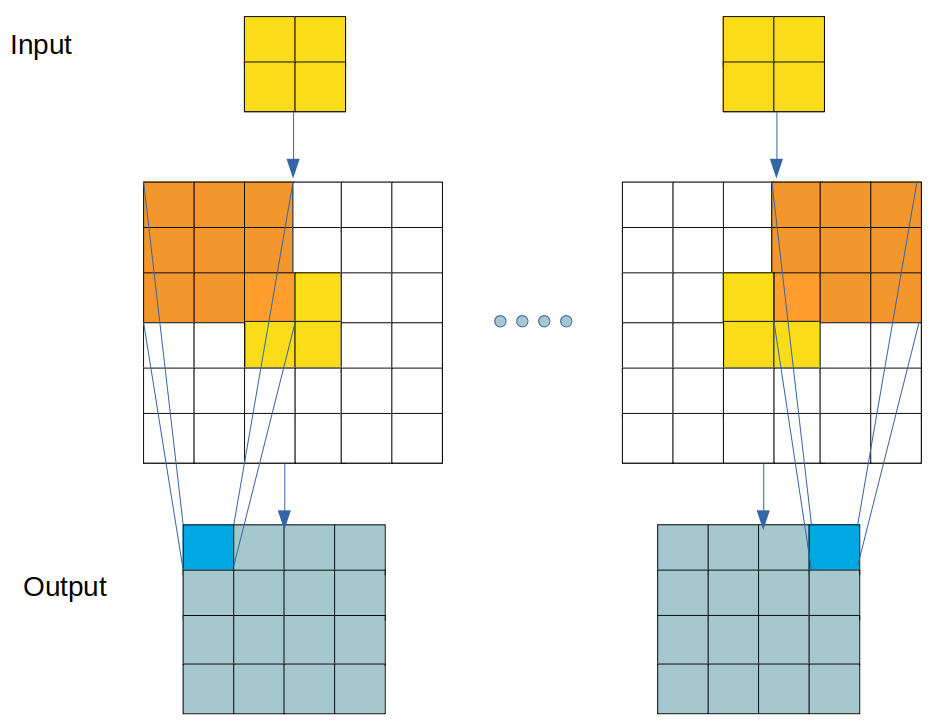
\includegraphics[width=5.5cm]{figure/transposedconv-2.png}
\caption{\textbf{Transposed} convolution as a regular convolution: with $k'=3, s'=1, p'=2$, dimensionality re-increases from $2\times 2$ to $4\times 4$.}
\end{figure}
\framebreak

\begin{itemize}
\item In general: a convolution with kernel $k$, stride $s$, padding $p$ has an associated transposed convolution with $k'=k$, $s'=s$, $p'=k-1$.
\end{itemize}
\framebreak
Convolution as matrix multiplication:
\begin{figure}
\centering
\scalebox{0.75}{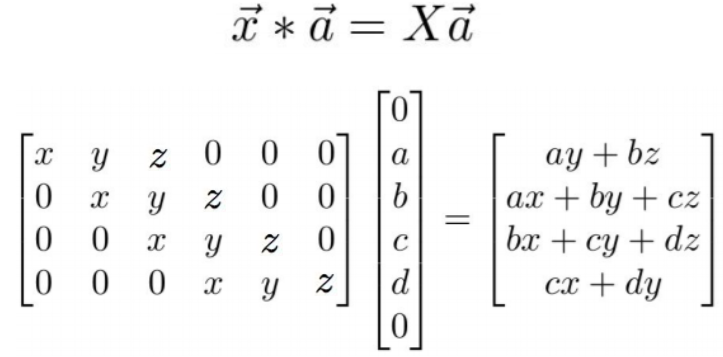
\includegraphics{figure/transpose_mat_1.png}}
\tiny{\\(Li, 2023)}
\caption{A regular 1D convolution, stride 1, padding 1. Vector $a$ is the 1D input feature map.}
\end{figure}
\framebreak
Transposed convolution as matrix multiplication:
\begin{figure}
\centering
\scalebox{0.6}{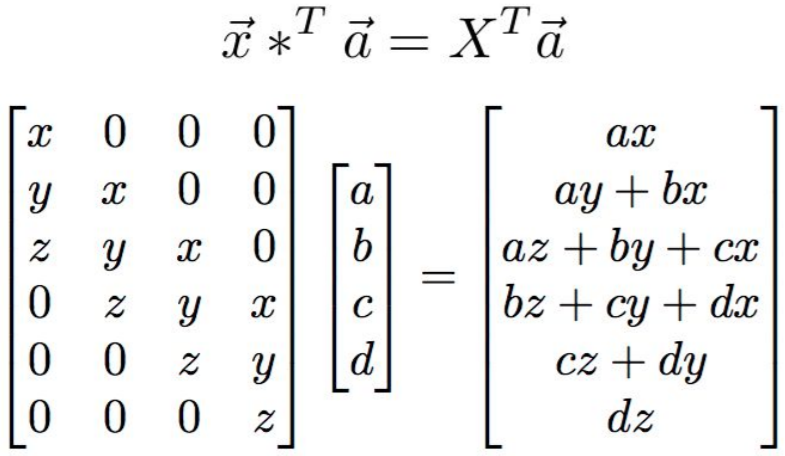
\includegraphics{figure/transpose_mat_2.png}}
\tiny{\\(Li, 2023)}
\caption{Upsampling a length-4 vector to length-6, stride 1. Note the change in padding.}
\end{figure}
\small{Important: even though the matrix structure here is the transpose of the original, its non-zero elements are, in general, different --- these are tuned by backpropagation, not derived analytically.}
\end{vbframe}
%%%%%%%%%%%%%%%%%%%%%%%%%%%%%%%%%%%%%%%%%%%

\begin{frame}{Transposed Convolutions --- A Different View}
  \only<1>{
  \begin{figure}
      \centering
      \scalebox{0.9}{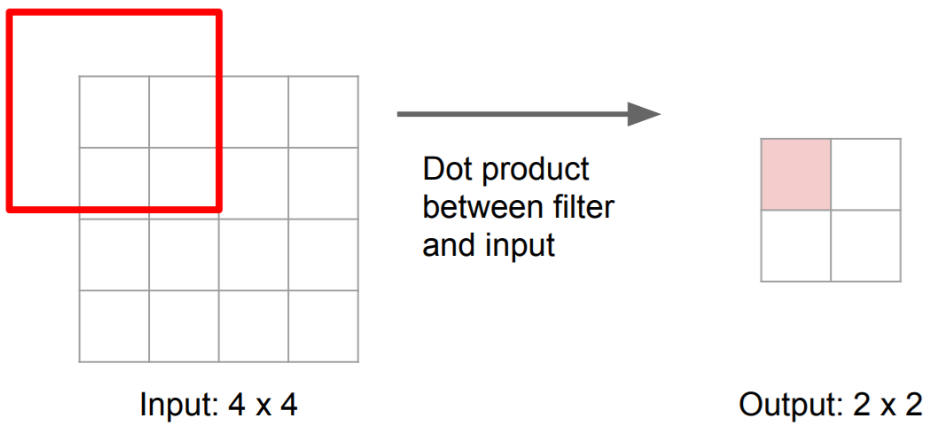
\includegraphics{figure/tr_conv_1.png}}
      \caption{Regular $3\times 3$ convolution, stride 2, padding 1 (Li, 2023).}
  \end{figure}
 }
  \only<2>{
  \begin{figure}
      \centering
      \scalebox{0.9}{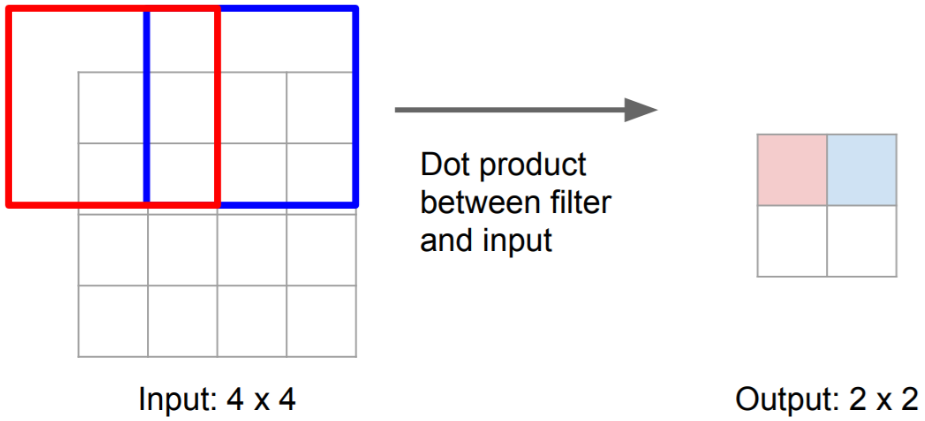
\includegraphics{figure/tr_conv_2.png}}
      \caption{Regular $3\times 3$ convolution, stride 2, padding 1 (Li, 2023).}
  \end{figure}
 }
  \only<3>{
  \begin{figure}
      \centering
      \scalebox{0.8}{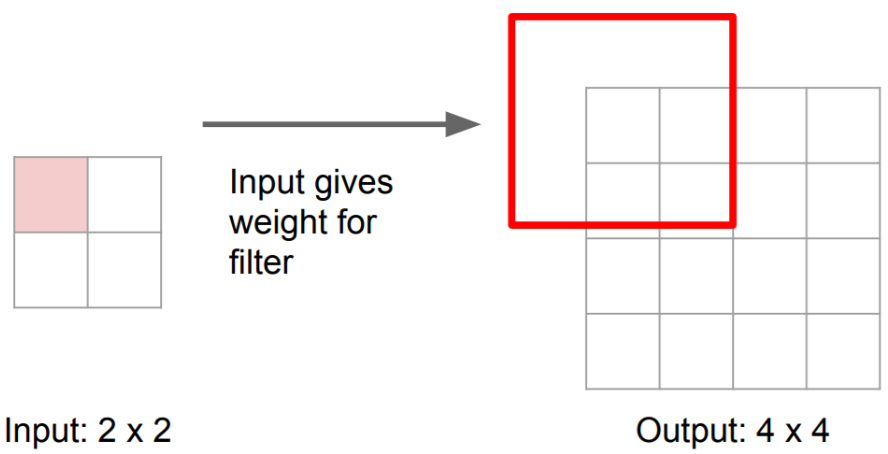
\includegraphics{figure/tr_conv_3.png}}
      \caption{\textit{Transposed} $3\times 3$ convolution, stride 2, padding 1. Stride now refers to the \textit{output} (Li, 2023).}
  \end{figure}
   Here, the filter is \textit{scaled} by the input.
 }
  \only<4>{
  \begin{figure}
      \centering
      \scalebox{0.8}{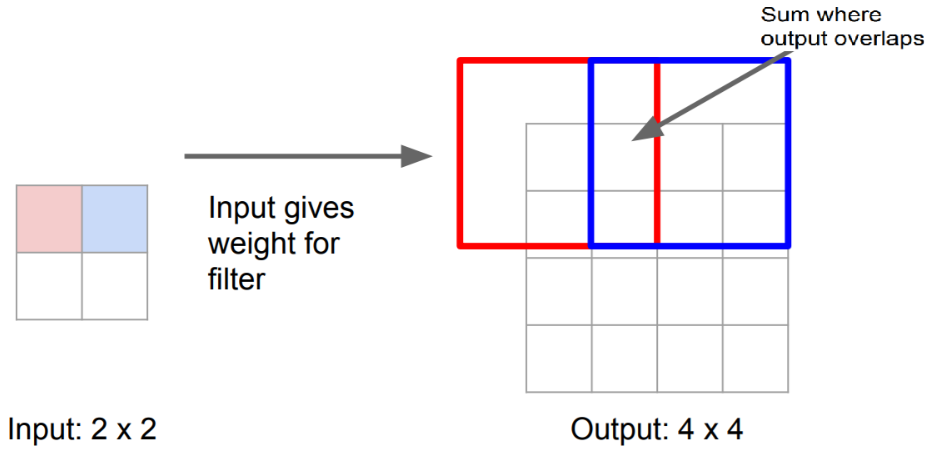
\includegraphics{figure/tr_conv_4.png}}
      \caption{\textit{Transposed} $3\times 3$ convolution, stride 2, padding 1. Stride now refers to the \textit{output} (Li, 2023).}
  \end{figure}
  Here, the filter is \textit{scaled} by the input.
 }
\end{frame}
%%%%%%%%%%%%%%%%%%%%%%%%%%%%%%%%%%%%%%

\begin{frame}{Transposed Convolutions --- A Drawback}
    \begin{figure}
        \centering
        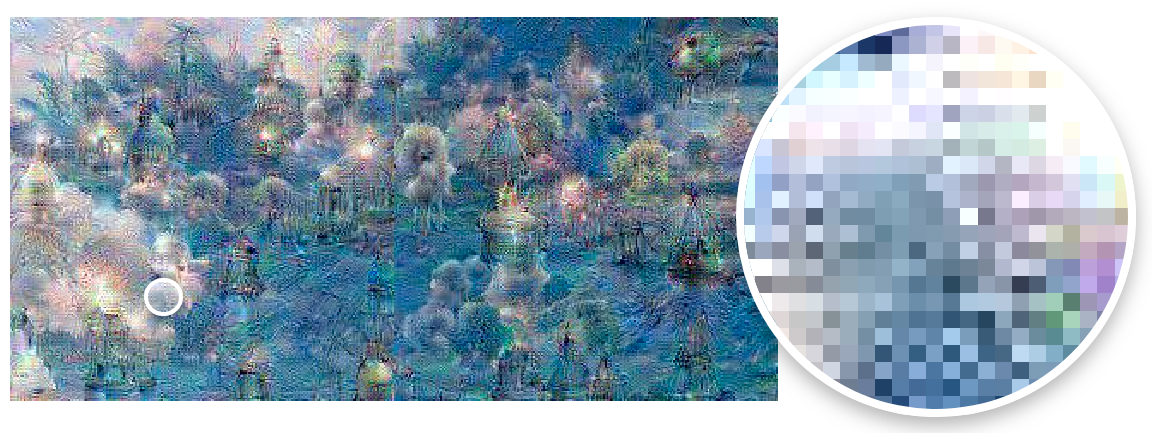
\includegraphics[width=8cm]{figure/transpose_artifact.png}
        \caption{Checkerboard-style artifacts produced by transposed convolutions (Odena et al., 2016).}
    \end{figure}
    \begin{itemize}
        \item Explanation: transposed convolution creates uneven overlap between some feature-map values, giving them higher magnitude than others --- the checkerboard pattern.
    \end{itemize}
\end{frame}
%%%%%%%%%%%%%%%%%%%%%%%%%%%%%%%%%%%%%%%%%%%

\begin{frame}{Transposed Convolutions --- A Drawback}
        \begin{figure}
            \centering
              \scalebox{0.65}{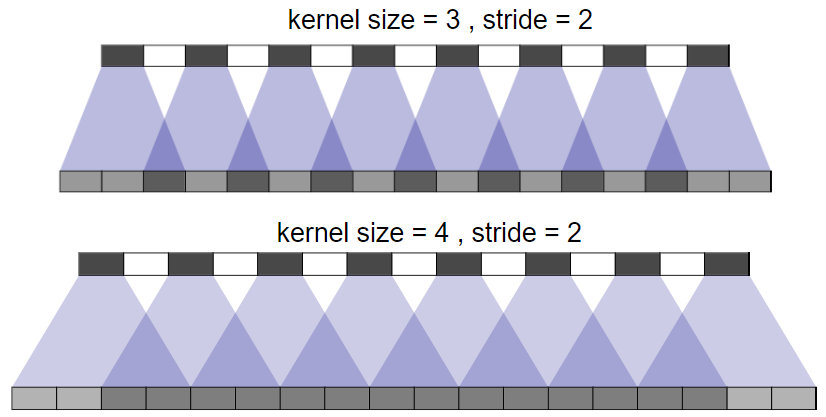
\includegraphics{figure/deconv_blog.png}}
            \caption{\footnotesize{1D example (top = input, bottom = output). \textit{Top}: uneven kernel overlap creates a checkerboard pattern. \textit{Bottom}: no checkerboard, because kernel size is divisible by stride (Odena et al., 2016).}}
        \end{figure}
    \begin{itemize}
         \item Solutions: upsample first (bilinear / nearest-neighbor) then apply a regular convolution; or ensure the kernel size is divisible by the stride.
     \end{itemize}
\end{frame}
%%%%%%%%%%%%%%%%%%%%%%%%%%%%%%%%%%%%%%%%%%%

\begin{frame}{Transposed Convolutions --- A Drawback}
     \begin{figure}
         \centering
         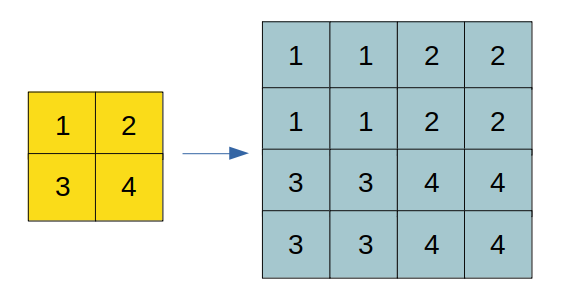
\includegraphics[width=7cm]{figure/transposedconv-last.png}
         \caption{Nearest-neighbor upsampling followed by a same convolution avoids checkerboard artifacts.}
     \end{figure}
\end{frame}
%%%%%%%%%%%%%%%%%%%%%%%%%%%%%%%%%%%%%%%%%%%
%%%%%%%%%%%%%%%%%%          REFERENCES          %%%%%%%%%%%%%%%%%%
%%%%%%%%%%%%%%%%%%%%%%%%%%%%%%%%%%%%%%%%%%%%%%%%%%%%%%%%%%%%%%%%%%
\begin{vbframe}
\frametitle{References}
\footnotesize{
\begin{thebibliography}{99}
\bibitem[(Roy, 2019)]{1} Roy, R. (2019, February 4). \textit{Temporal Convolutional Networks}. Medium. \url{https://medium.com/@raushan2807/temporal-convolutional-networks-bfea16e6d7d2}
\bibitem[(Li, 2023)]{2} Li, F.-F. (2023). \textit{Lecture 11: Detection and segmentation --- Stanford University}. CS231n. \url{http://cs231n.stanford.edu/slides/2017/cs231n_2017_lecture11.pdf}
\bibitem[(Odena et al., 2016)]{3} Odena, A., Dumoulin, V., \& Olah, C. (2016, October 17). \textit{Deconvolution and checkerboard artifacts}. Distill. \url{https://distill.pub/2016/deconv-checkerboard/}
\end{thebibliography}
}
\end{vbframe}

%%%%%%%%%%%%%%%%%%%%%%%%%%%%%%%%%%%%%%%%%%%%%%%%%%%%%%%%%%%%%%%%%%
\section{Pooling}
%%%%%%%%%%%%%%%%%%%%%%%%%%%%%%%%%%%%%%%%%%%%%%%%%%%%%%%%%%%%%%%%%%

\begin{frame}{Max Pooling}
\center
\only<1>{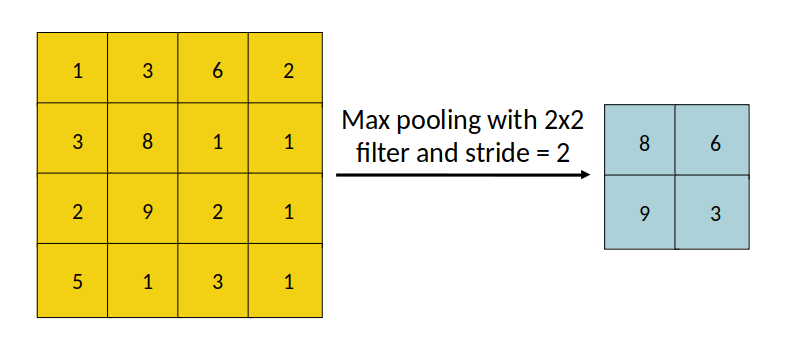
\includegraphics[width=10cm]{figure/maxpool1.png}}
\only<2>{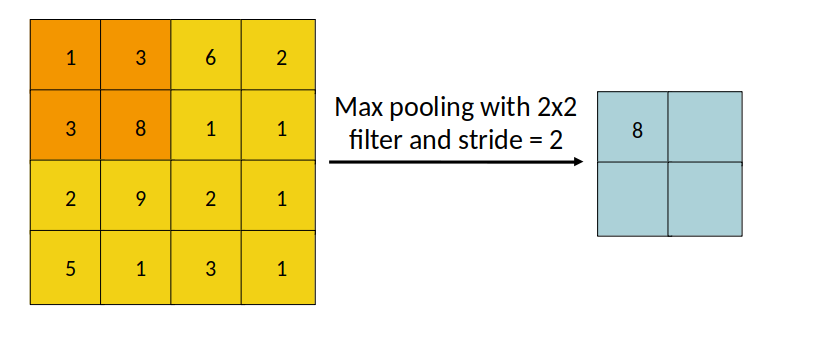
\includegraphics[width=10cm]{figure/maxpool2.png}}
\only<3>{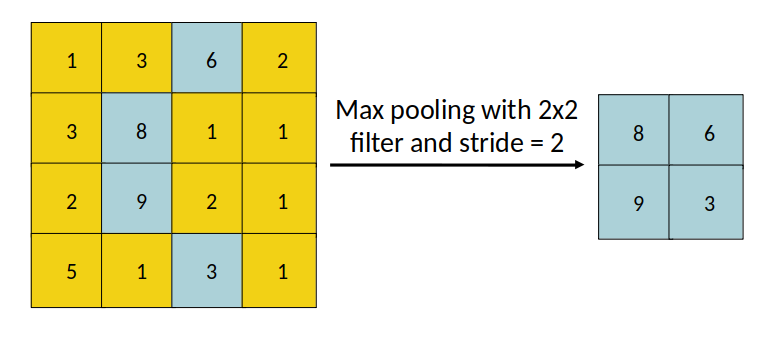
\includegraphics[width=10cm]{figure/maxpoolend.png}}
\begin{itemize}
\only<1>{\item We've seen how convolutions work --- there is one more operation to understand: we want to downsample the feature map while ideally losing no information.}
\only<2>{\item Max pooling looks for the maximum value at each spatial location --- here, 8 for the first location. With a filter of size 2 and no padding, we get a downsampled result.}
\only<3>{\item The final pooled feature map has entries 8, 6, 9, 3. Max pooling brings two properties: dimensionality reduction and (limited) spatial invariance.
\item Popular pooling functions: max and (weighted) average.}
\end{itemize}
\end{frame}
%%%%%%%%%%%%%%%%%%%%%%%%%%%%%%%%%%%%%%%%%%%%%%%%%%%%%%%%%%%%%%%%%%

\begin{frame}{Average Pooling}
\center
\only<1>{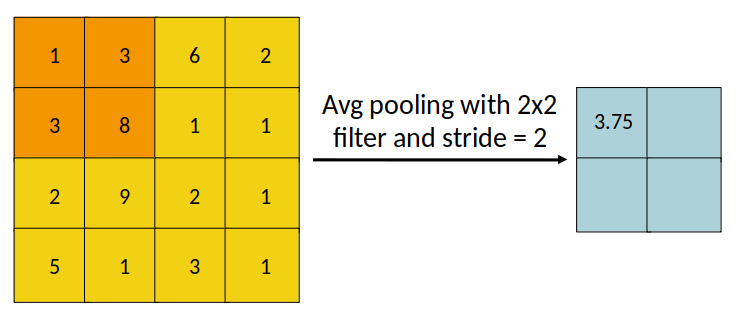
\includegraphics[width=10cm]{figure/avgpool1.png}}%
\only<2>{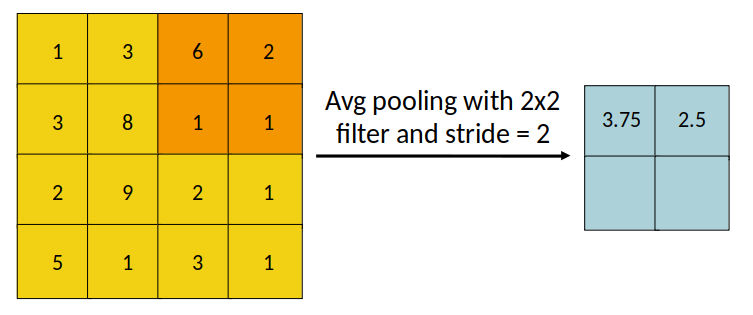
\includegraphics[width=10cm]{figure/avgpool2.png}}%
\only<3>{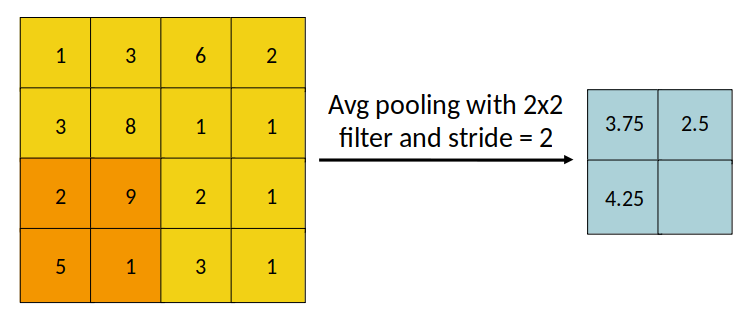
\includegraphics[width=10cm]{figure/avgpool3.png}}%
\only<4>{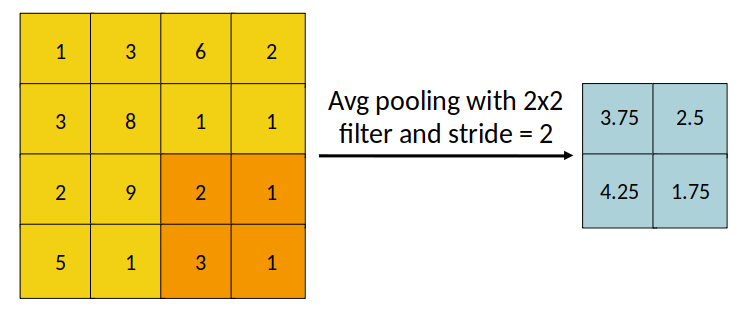
\includegraphics[width=10cm]{figure/avgpool4.png}}%
\begin{itemize}
\only<1>{\item Other pooling operations exist too: average, fractional, LP, softmax, stochastic, blur, global average pooling, and more. Like max pooling, average pooling downsamples the feature map, but may preserve more information.}
\only<2>{\item Average pooling takes the mean value at each spatial location.}
\only<3>{\item It uses all inputs (via the sum) and backpropagates to all of them --- but is less robust to noise than max pooling.}
\only<4>{\item The final pooled feature map has entries 3.75, 2.5, 4.25, 1.75.}
\end{itemize}
\end{frame}
%%%%%%%%%%%%%%%%%%%%%%%%%%%%%%%%%%%%%%%%%%%%%%%%%%%%%%%%%%%%%%%%%%

\begin{vbframe}{Comparison of Max and Average Pooling}
\begin{itemize}
\item Average pooling uses the information of all inputs; max pooling uses only the largest value.
\item Max pooling removes detail, so it suits sparse information (typically image classification); average pooling suits dense information (typically NLP).
\end{itemize}
\begin{figure}
\centering
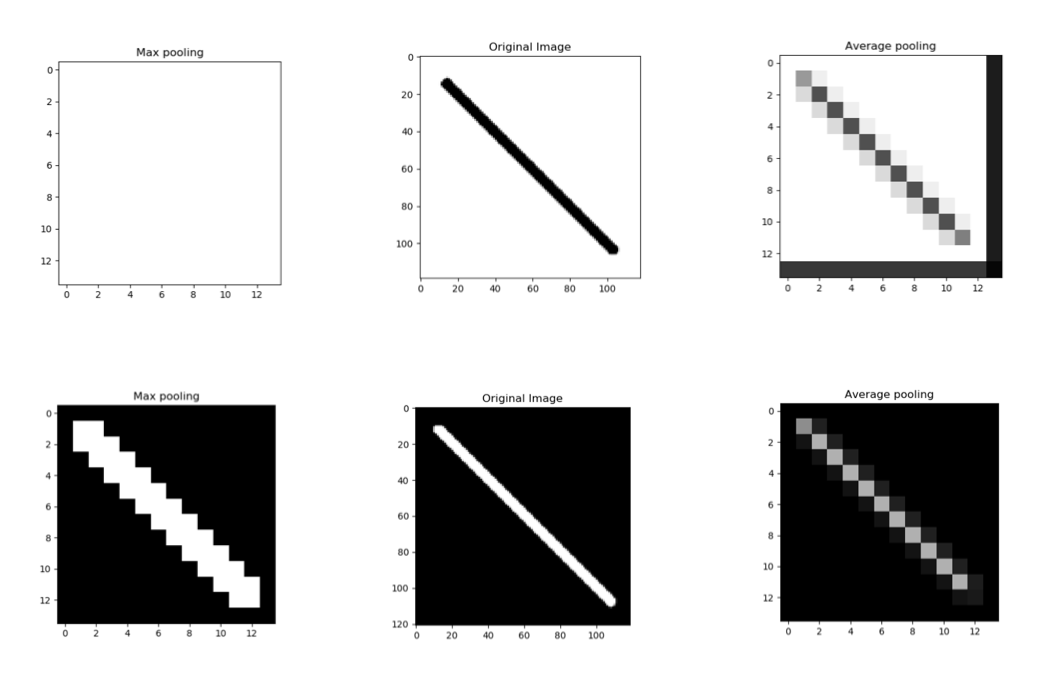
\includegraphics[width=5cm]{figure/pooling.png}
\caption{Shortcomings of max and average pooling on a toy image (Sharma, 2020).}
\end{figure}
\end{vbframe}
%%%%%%%%%%%%%%%%%%%%%%%%%%%%%%%%%%%%%%%%%%%%%%%%%%%%%%%%%%%%%%%%%%
%%%%%%%%%%%%%%%%%%          REFERENCES          %%%%%%%%%%%%%%%%%%
%%%%%%%%%%%%%%%%%%%%%%%%%%%%%%%%%%%%%%%%%%%%%%%%%%%%%%%%%%%%%%%%%%
\begin{vbframe}
\frametitle{References}
\footnotesize{
\begin{thebibliography}{99}
\bibitem[(Sharma, 2020)]{1} Sharma, P. (2020, April 21). \textit{MaxPool vs AvgPool}. OpenGenus IQ. \url{https://iq.opengenus.org/maxpool-vs-avgpool/}
\end{thebibliography}
}
\end{vbframe}

%%%%%%%%%%%%%%%%%%%%%%%%%%%%%%%%%%%%%%%%%%%%%%%%%%%%%%%%%%%%%%%%%%
\section{Modern Architectures}
%%%%%%%%%%%%%%%%%%%%%%%%%%%%%%%%%%%%%%%%%%%%%%%%%%%%%%%%%%%%%%%%%%

\begin{vbframe}{From LeNet to Modern CNNs}
A brief tour of how the field evolved, without going deep on any single architecture:
  \begin{itemize}
    \item \textbf{LeNet} (LeCun, 1998): the first practical CNN, applied to handwritten-digit recognition (MNIST); depth was mainly limited by 1990s compute.
    \item \textbf{AlexNet} (2012): 8 layers, ReLU instead of sigmoid, won ImageNet (ILSVRC) by a huge margin --- the result that triggered the deep learning boom in vision.
    \item \textbf{VGG} (2014): showed that stacking many small $3\times 3$ filters (rather than fewer, larger ones) with more depth improves performance, and introduced the reusable \enquote{block} as a network-design unit.
    \item \textbf{GoogLeNet / Inception} and \textbf{Network-in-Network}: parallel filter paths of different sizes plus $1\times 1$ convolutions to control channel depth cheaply; global average pooling replaces huge dense layers, cutting parameters and overfitting.
    \item \textbf{ResNet} (2015): simply stacking more layers made networks \emph{harder} to train, not easier. The fix --- \textbf{skip connections}, letting a layer default to the identity function --- is important and general enough to cover in depth next.
    \item \textbf{DenseNet}: pushes the skip-connection idea further by concatenating every layer's output into all subsequent layers, not just adding it.
    \item \textbf{U-Net}: a convolutional encoder--decoder using skip connections between mirrored layers --- the workhorse of image segmentation.
  \end{itemize}
\end{vbframe}
%%%%%%%%%%%%%%%%%%%%%%%%%%%%%%%%%%%%%%%%%%%%%%%%%%%%%%%%%%%%%%%%%%

\begin{vbframe}{Residual Networks: Why Skip Connections?}
Problem setting: in principle, stacking more layers should never hurt --- a network could always learn to make extra layers the identity function and skip them.
 \begin{figure}
  \centering
    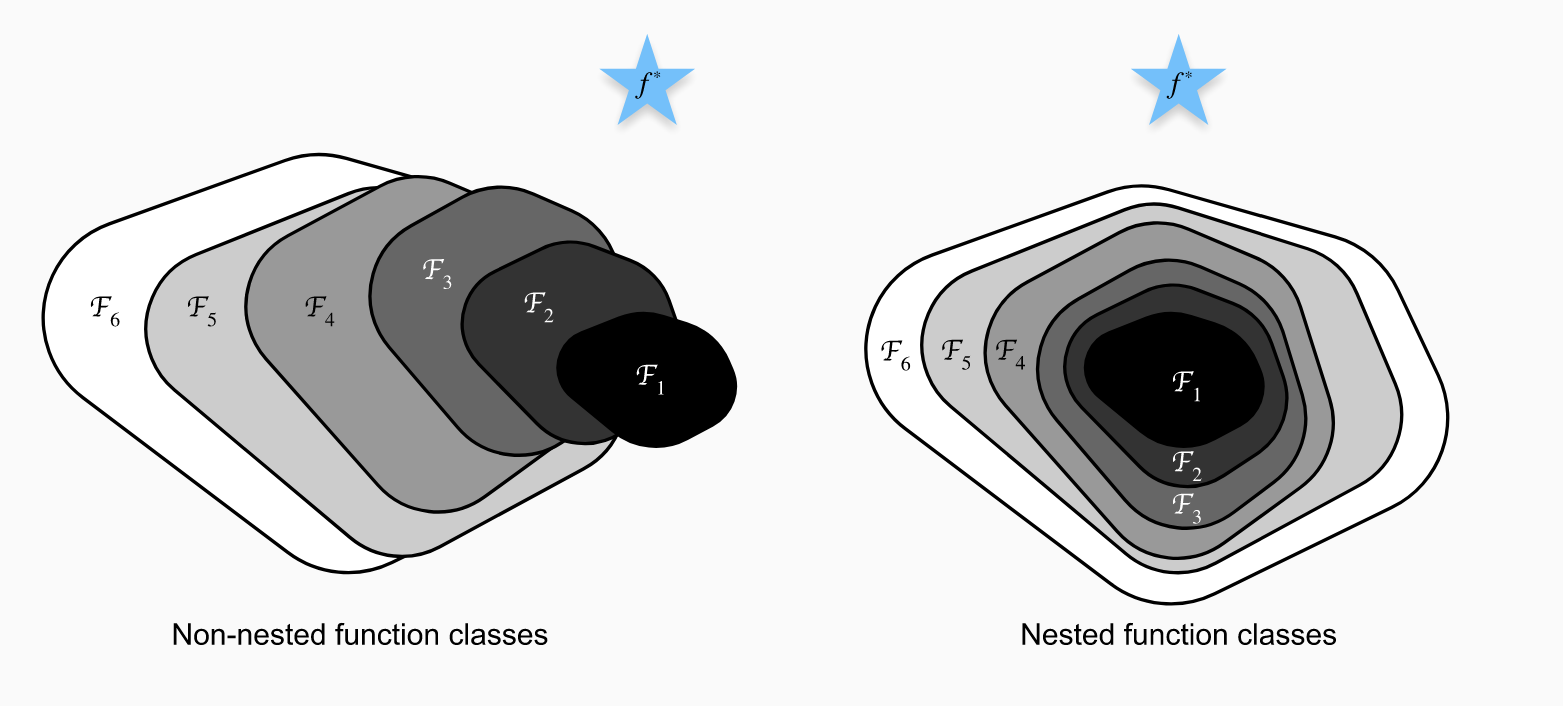
\includegraphics[width=8cm]{figure/resnet_problem.png}
    \caption{For non-nested function classes, a larger function class need not get closer to the true function $\mathcal{F}^*$ --- this does not happen for nested function classes (Dive into Deep Learning).}
  \end{figure}
    \begin{itemize}
        \item In practice: learning an identity mapping $\xv = \mathcal{F}(\xv)$ through many nonlinear layers is hard, and simply stacking more layers increased \emph{both} train and test error (not overfitting).
        \item Introduced by He et al.\ (2015): give the model an explicit shortcut to skip layers that aren't useful.
    \end{itemize}
\framebreak
 \begin{figure}
  \centering
    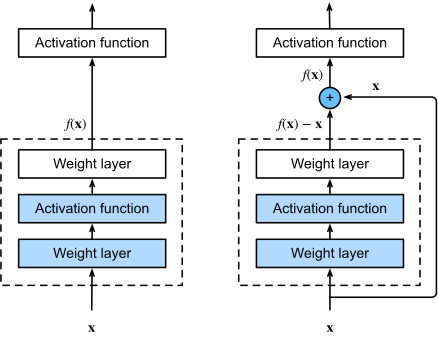
\includegraphics[width=7cm]{figure/residual-block.png}
    \caption{A regular block (left) vs.\ a residual block (right): the input is added back via an identity (skip) connection (Dive into Deep Learning).}
  \end{figure}
    \begin{itemize}
        \item Let $\mathcal{H}(\xv)$ be the mapping a layer should learn. Instead of fitting $\mathcal{H}(\xv)$ directly, the layer fits the \textbf{residual} $\mathcal{F}(\xv) := \mathcal{H}(\xv) - \xv$, while $\xv$ is added back via the identity: $\mathcal{H}(\xv) = \mathcal{F}(\xv) + \xv$.
        \item The residual mapping can push weights toward zero to approximate the identity --- much easier than learning it directly through nonlinear activations.
    \end{itemize}
\end{vbframe}
%%%%%%%%%%%%%%%%%%%%%%%%%%%%%%%%%%%%%%%%%%%%%%%%%%%%%%%%%%%%%%%%%%

\begin{frame}{Residual Networks: Why It Mattered}
    \begin{itemize}
        \item Inputs and gradients can flow through the identity path even in very deep networks, letting ResNets train reliably at depths (e.g.\ ResNet-50/101/152) where plain stacked networks degrade.
        \item ResNet had a major influence on the design of later networks, convolutional and sequential alike.
        \item Skip connections became a default building block far beyond CNNs --- they reappear inside Transformer blocks, covered in Session 7. That's a running theme of this course: a mechanism can outlive the specific architecture it was introduced in, which is exactly why we spend a full session on Transformers next.
    \end{itemize}
\end{frame}
%%%%%%%%%%%%%%%%%%%%%%%%%%%%%%%%%%%%%%%%%%%%%%%%%%%%%%%%%%%%%%%%%%
%%%%%%%%%%%%%%%%%%          REFERENCES          %%%%%%%%%%%%%%%%%%
%%%%%%%%%%%%%%%%%%%%%%%%%%%%%%%%%%%%%%%%%%%%%%%%%%%%%%%%%%%%%%%%%%
\begin{vbframe}
\frametitle{References}
\footnotesize{
\begin{thebibliography}{99}
\bibitem[(Dive into Deep Learning)]{1} Dive into Deep Learning. (n.d.). \textit{8.6. Residual Networks (ResNet) and ResNeXt}. \url{http://d2l.ai/chapter_convolutional-modern/resnet.html}
\bibitem[(He et al., 2015)]{2} He, K., Zhang, X., Ren, S., \& Sun, J. (2015). \textit{Deep Residual Learning for Image Recognition}. \url{https://arxiv.org/abs/1512.03385}
\end{thebibliography}
}
\end{vbframe}

%%%%%%%%%%%%%%%%%%%%%%%%%%%%%%%%%%%%%%%%%%%%%%%%%%%%%%%%%%%%%%%%%%
\section{License \& Attribution}
%%%%%%%%%%%%%%%%%%%%%%%%%%%%%%%%%%%%%%%%%%%%%%%%%%%%%%%%%%%%%%%%%%

\begin{vbframe}{License \& Attribution}
\begin{itemize}
\item Basic Concepts, The Convolution Operation, 1D/2D/3D Convolutions, CNN Components,
Properties of Convolution, Dilated and Transposed Convolutions, and Pooling adapted from
\textbf{Introduction to Deep Learning (I2DL)}, Prof.\ Dr.\ Bernd Bischl, SLDS, LMU Munich.
\url{https://github.com/slds-lmu/lecture_i2dl} --- licensed \textbf{CC BY 4.0}:
\url{https://creativecommons.org/licenses/by/4.0/}
\item Modern Architectures adapted (and substantially condensed) from the same I2DL source
(\texttt{slides/cnn3/}) --- also licensed \textbf{CC BY 4.0}.
\item Content in this deck has been merged, reordered, and (for Modern Architectures)
substantially condensed from the originals; not used verbatim.
\end{itemize}
\end{vbframe}

\endlecture
\end{document}
